\externaldocument{Introduction.tex}
\externaldocument{Experimental_Apparatus.tex}
\externaldocument{Results.tex}
\externaldocument{Analysis.tex}
\externaldocument{EIC_Jets.tex}
\externaldocument{Discussion.tex}
\chapter{Introduction}

\section{QCD}
\label{sec:QCD}
Quantum Chromodynamics (QCD) is the fundamental theory of the strong nuclear interaction. The QCD lagrangian characterizing this interaction is~\cite{and2010}:

% \[
%   \mathcal{L}_\mathrm{QCD} = \bar{\psi}_i\left(i\gamma^\mu\delta_\mu-m_i\right)\psi_j - gG_\mu^\alpha \bar{\psi}_i\gamma^\mu\mathcal{T}_{ij}^\alpha\psi_i- \frac{1}{4}G^a_{\mu \nu} G^{\mu \nu}_a
% .\] 

\begin{equation}
  \mathcal{L}_\mathrm{QCD} = \sum_q \bar{\psi}_{q,a}\left(i\gamma^\mu\partial_\mu \delta_{ab} -g_s\gamma^\mu t^{C}_{ab} \mathcal{A}_\mu^C - m_q\delta_{ab}\right) \psi_{q,b} - \frac{1}{4}F^\mathcal{A}_{\mu\nu}F^{\mathcal{A}\mu\nu},
\label{eq:qcd_lagrangian}
\end{equation} 

The QCD lagrangian is strikingly similar the QED lagrangian which details the electromagnetic interaction. In both cases, $\psi$ represents the field of a spin $\frac{1}{2}$ fermion. In QCD, this fermion is called a \textit{quark}. $\mathcal{A}$ represents the field of the massless spin-1 boson called the \textit{gluon}, which couples to the fermion field with strength $g_s$. Quarks and gluons are the fundamental components of the \textit{parton model}, and together make up all composite hadrons such as protons, neutrons an pions.

$F$ represents the gluon field strength tensor, and is analogous to the electromagnetic field strength tensor. It can be expressed in terms of the gluon field, $\mathcal{A}$, as:

\begin{equation}
  F^a_{\mu \nu} = \partial_\mu \mathcal{A}^a_\nu - \partial_\nu \mathcal{A}^a_\mu + g_s f^{abc} \mathcal{A}^b_\mu \mathcal{A}^c_\nu.
\label{eq: gluon_tensor}
\end{equation}

Notably, the final term of this expansion represents the self-interaction of the gluon field, and has no analogous term in QED. The self-interaction of the gluon field fundamentally differentiates QCD from QED, and is responsible for the qualitatively different nature of matter at the sub-nuclear and atomic scales.

The SU(3) group mathematically describes the fundamental symmetries of QCD. Put another way, QCD is the SU(3) component of the $\mathrm{SU(3)}\times\mathrm{SU(2)}\times\mathrm{U(1)}$ Standard Model of Particle Physics. In the language of group theory, $t_{ab}^C$ represents the generators of the SU(3) group. They are a set of eight $3\times3$ matrices closely related to the Gell-Mann matrices: $t_{ab}^C = \lambda_{ab}^C/2$. $f^{abc}$ are the set of constants which satisfy the commutation relations of the generations, $[t^A,t^B] = if_{abc}t^C$. $\gamma^\mu$ are dirac $\gamma$ matrices.
But what aspect of our observable reality does the this group relate to? Physically, the SU(3) group corresponds to a theory containing the quantum number of color, the QCD analog of electric charge which can take three values, i.e. there are 3 colors. The theory also contains the quantum number for flavor, subscript \textit{q} in the lagrangian. Flavor \textit{q} can take on six different values indicating that there are six flavors of quarks, each with a mass and  fractional electric charge. Additionally, the eight generators of the SU(3) group indicate that there are in fact eight types of gluons, indexed with $C$ in Eq.~\ref{eq:qcd_lagrangian}.
 
Both QCD and QED are characterized by a scale dependant coupling. This means that the strength of the coupling depends on the momentum exchange. In QCD, this coupling is labelled $\alpha_S$, 
and is defined as  $\alpha_S \equiv g_S^2/4\pi$. The dependence of the 
coupling on momentum is encoded in the beta function which is expanded as a perturbative series in $\alpha_S$:

\begin{equation}
  \beta(\alpha_S) = b\alpha_S^2+\mathcal{O}(\alpha_S^3) 
  \label{eq:beta}
\end{equation}

This $\beta$ function was evaluated in 1973 by Gross, Wilczek, and Politzer, \cite{Gross1973,Politzer1973}where they famously found:

  \begin{equation}
    b =  -\frac{33 - 2n_f}{12\pi} 
    \label{eq:b}
  \end{equation}

with $n_f$ as the number of quark flavors. Using this result, the dependence of the strong interaction on the momentum scale, Q, is:

  \begin{equation}
    a_S(Q^2) = \frac{1}{b\log(Q^2/\Lambda^2)}
  \label{eq:a_S_running}
  \end{equation}

  Where $\Lambda$ defines the coupling scale at which perturbation theory breaks down and the series in  $\alpha_S$ no longer converges. $\Lambda$ has been measured experimentally to be  $\approx 200$MeV \cite{Bettini2008}. The running of the coupling is shown in Fig.~\ref{fig:a_S_running}
%A. Bettini, Introduction to Elementary Particle Physics (Cambridge University Press, 2008).

  \begin{figure}[htpb]
    \centering
    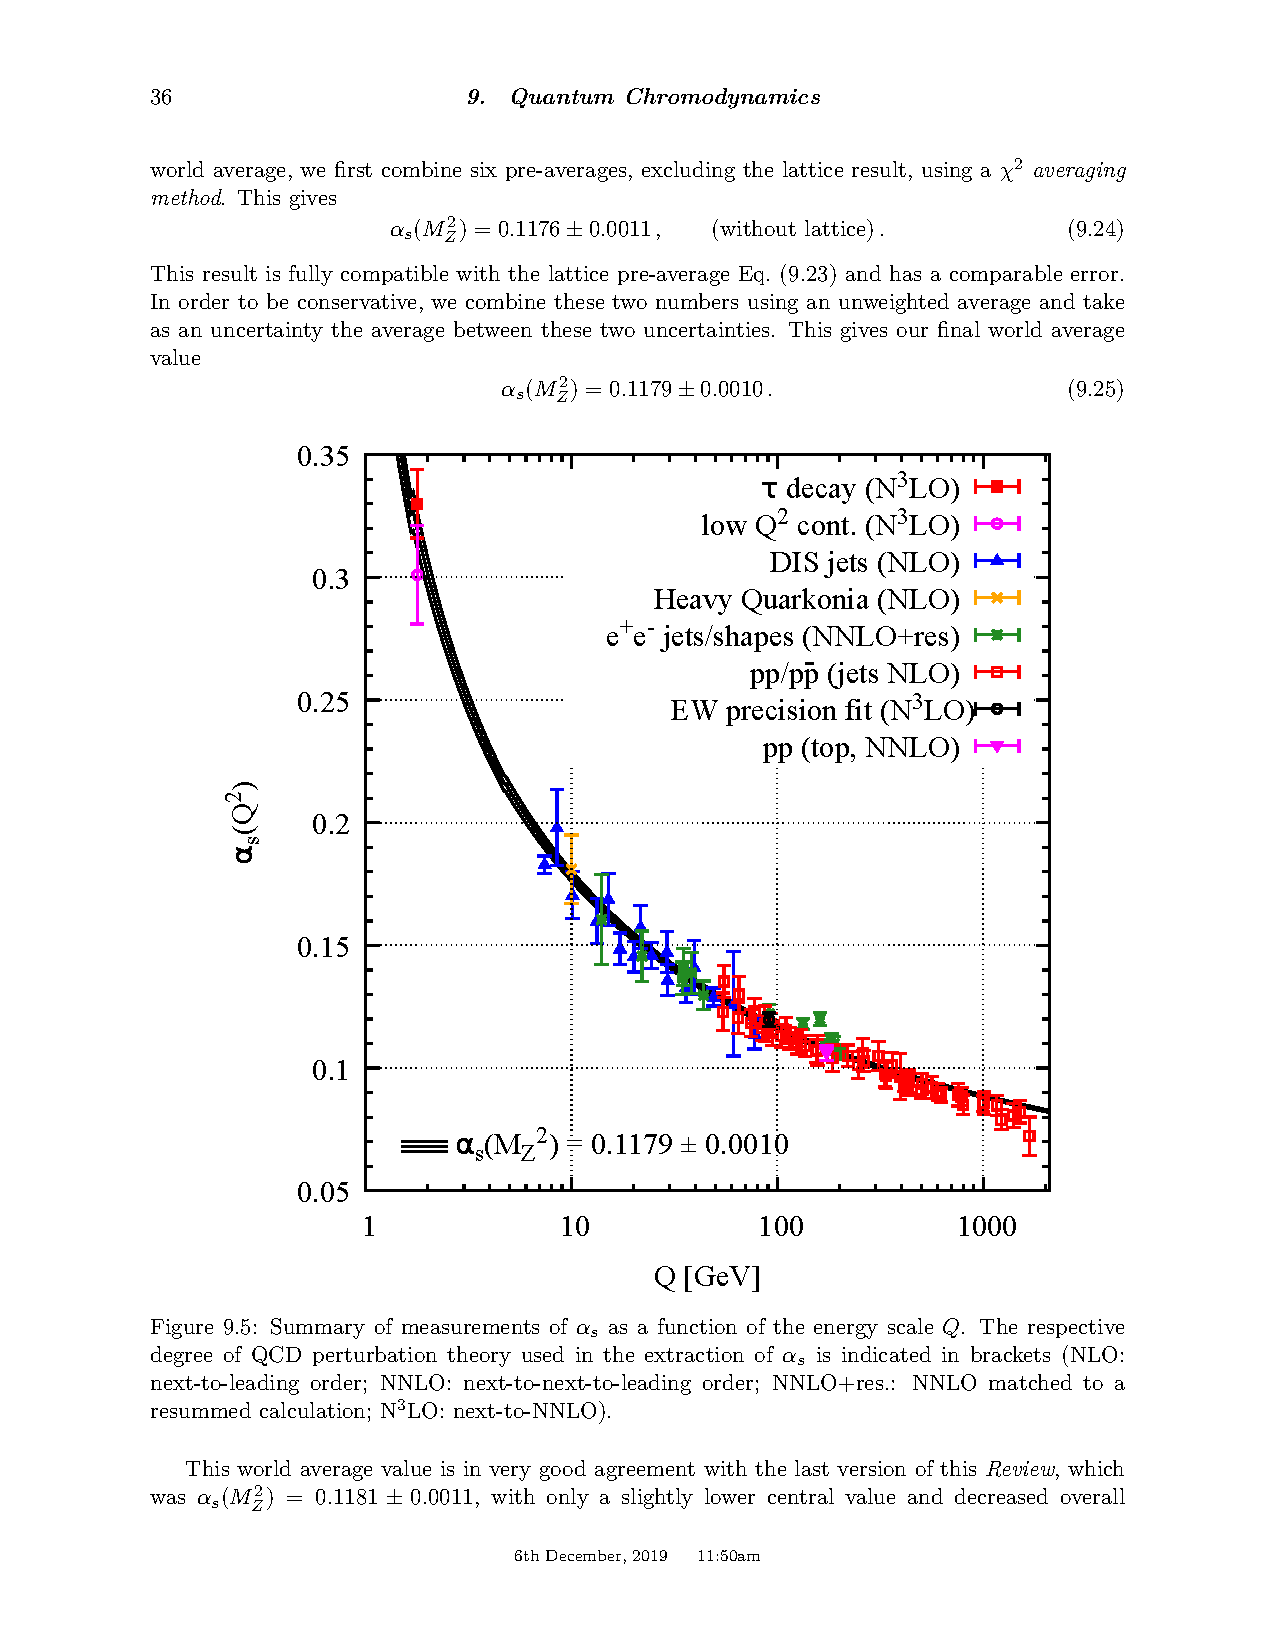
\includegraphics[trim={3.5cm 5.9cm 3cm 7cm},clip,width=1.0\textwidth] {Introduction/a_S_running.pdf}
    \caption{The QCD coupling constant, $\alpha_S$, plotted as a function of the momentum scale,  $Q$ for various measurements. The degree of perturbation theory used in the extraction of  $\alpha_S$ is indicated in brackets next to each measurement. The bottom left shows the global average for the coupling strength at the Z boson mass, $Q=M_Z$ \cite{zotero-314}.}
    \label{fig:a_S_running}
  \end{figure}
  

  Thus, we reach yet another important divergence from QED: While in QED, the coupling becomes larger at higher energy, the negative value of b in Eq.~\ref{eq:b} means that in QCD, the coupling becomes smaller at higher energy. This property is known as \textit{asymptotic freedom}, and indicates that at large energy, the interaction between quarks is small. 
  On the opposite end of the scale, for example when the distance between quarks grows large, the energy stored by the field exceeds the threshold for the creation of new matter (in the form of a $q\bar{q}$ pair). This phenomenon is know as \textit{confinement}, and results in the absence of free quarks in nature. They are instead trapped in bound states with a net zero color charge known as mesons containing a quark and an anti-quark, or baryons consisting of three (anti)quarks.

\section{Relativistic Heavy Ion Collisions}\label{sec:rhics}
% The study of high energy nuclear collisions may give us a more complete understanding of how particles are produced via QCD. But this is not a new endeaver, and is a natural extension of the question "how are particles produced in high-energy collisions?" A question that long predates even QCD.
Today, studying ultrarelativistic heavy ion collisions may give us a more complete understanding of how particles are produced in high-energy collisions via QCD, giving us a better understanding of one of the fundamental interactions of nature. The history of nuclear collisions, however, predates the parton model, and even QCD itself. The first dedicated heavy-ion accelerator, the Heavy Ion Linear Accelerator (HILAC) began operation in 1957 in Berkeley, CA. At the time, the primary objectives of the field were nuclear transmutation and the investigation of radiation damage to human tissue for space travel. HILAC could accelerate ions as heavy as Argon up to 10MeV \cite{AIP2014}. A few years later, Gell-Mann and Feynman's parton model was verified by deep inelastic scattering experiments at SLAC, but it was not until the 70's that the theory of QCD was steadily developed. The idea of asymptotic freedom was discovered by David Gross and Frank Wilczek, and independently by David Politzer in 1973, who would not share the nobel prize until 2004. Based on this idea, J. C. Collins and M. J. Perry of Cambridge predicted that at sufficiently high densities, long-range interactions would be effectively screened and nuclear matter would behave as an ideal gas of quarks and gluons \cite[Collins1975]. %Edward Shuryak and others would expand on these ideas using the machinery of finite temperature field theory to hot, dense matter.  
This would mark a fundamentally new state of matter, the Quark Gluon Plasma (QGP). The study of this state of matter has became one of the primary goals of nuclear physicists and has helped motivate the construction of several collider facilities: the AGS, SPS, RHIC, and the LHC. The latter of which is capable of colliding Lead ions with a center of mass energy per nucleon of 5.02 TeV. A considerable step up from Argon ions at 10MeV. Fig.~\ref{fig:collision_snapshot} shows snapshots of a PbPb collision at different times \cite{annurev-nucl}.

\begin{figure}[htpb]
  \centering
  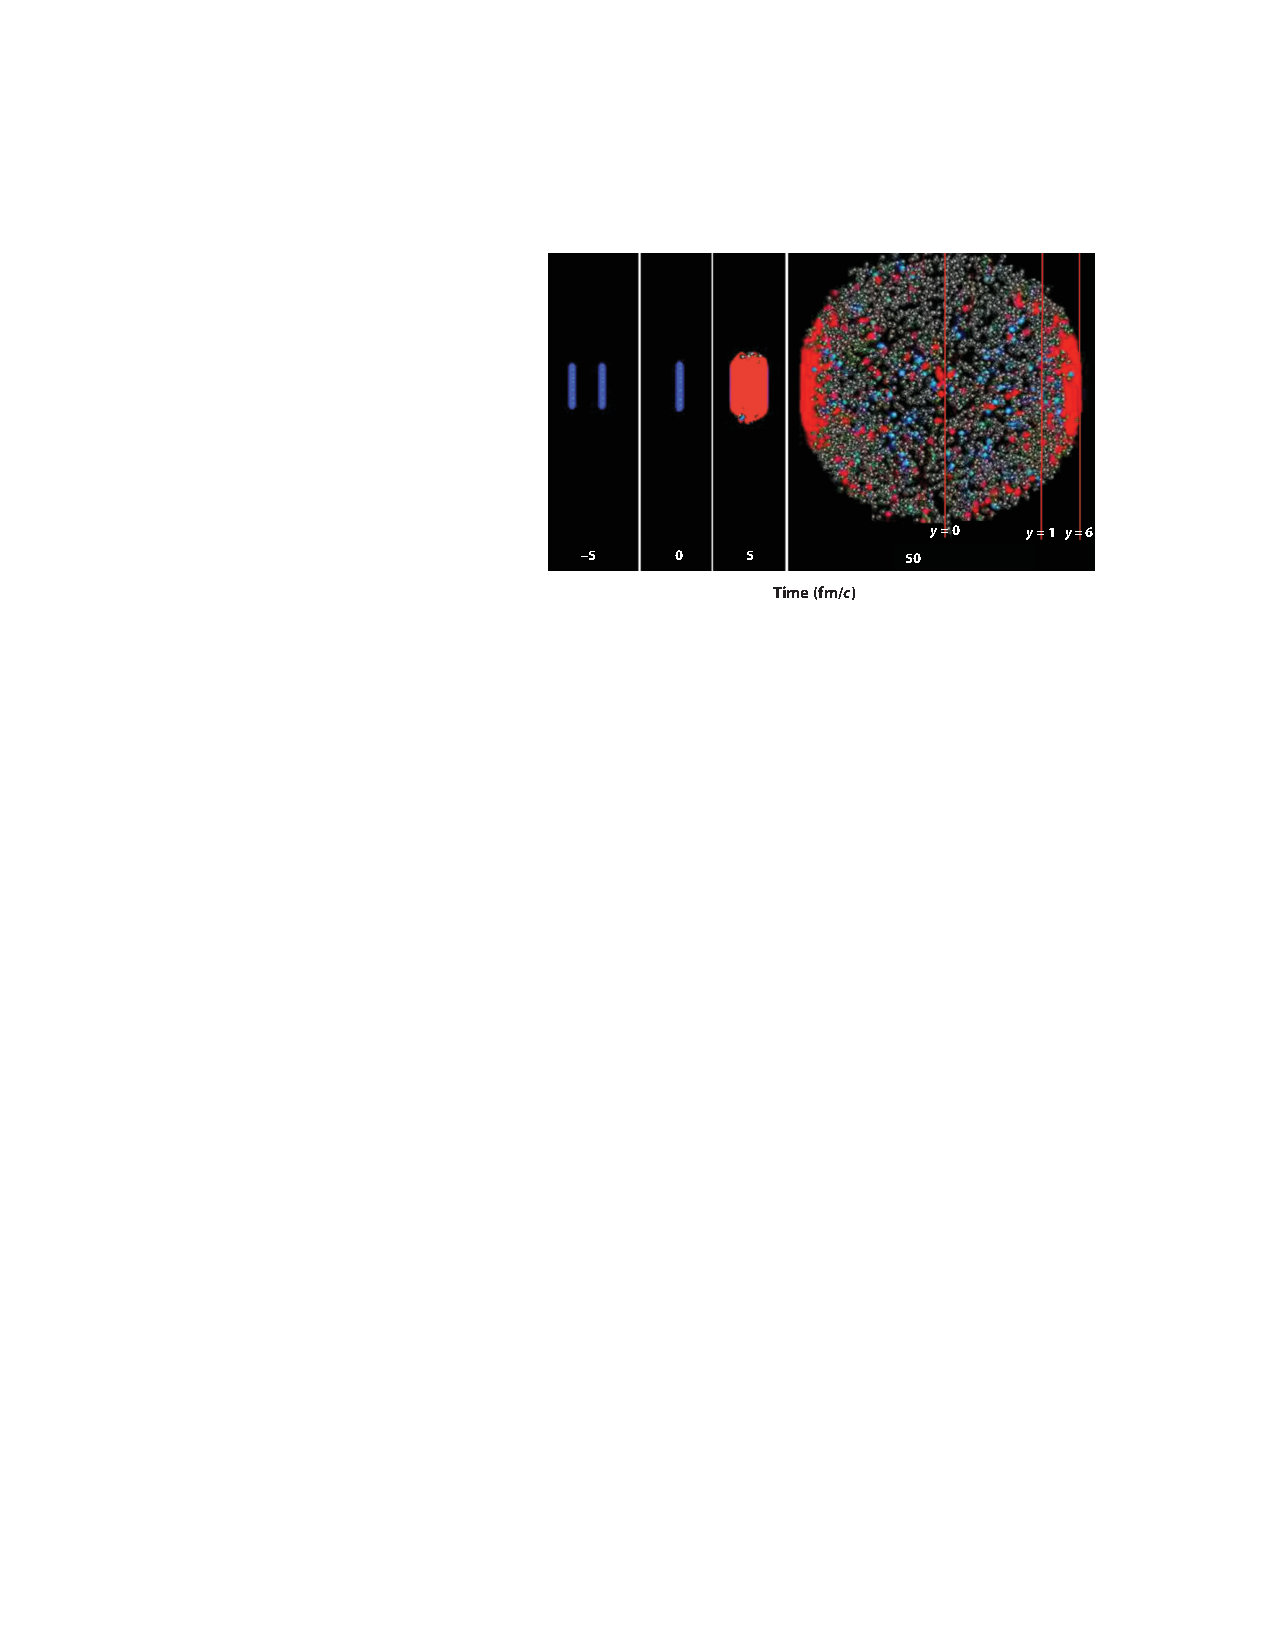
\includegraphics[width=0.99\textwidth]{Introduction/collision_snapshot.pdf}
  \caption{Snapshots of a central 2.76 TeV PbPb collision at different times with hadrons (blue and gray spheres) as well as quark gluon plasma (red). The red vertical lines indicate different regions of rapidity \cite{annurev-nucl}.}
  \label{fig:collision_snapshot}
\end{figure}

% \section{Properties and Signatures of Quark Gluon Plasma}\label{sec:QGP}

% QGP temperature. Because of this, observed modifications to observables attributed to the production of quark gluon plasma are often referred to as "hot nuclear matter effects".
\section{The Quark Gluon Plasma}\label{sec:QGP}

Investigating the QCD phase diagram as a function of both temperature and baryon doping (or net baryon number), is among one of the most important reasons for studying relativistic heavy ion collisions. Fig. \ref{fig:qcd_phase} shows the currently understood QCD phase diagram as a function of temperature and net baryon number, parametrized by the baryon chemical potential, $\mu_B$.

\begin{figure}[htpb]
  \centering
  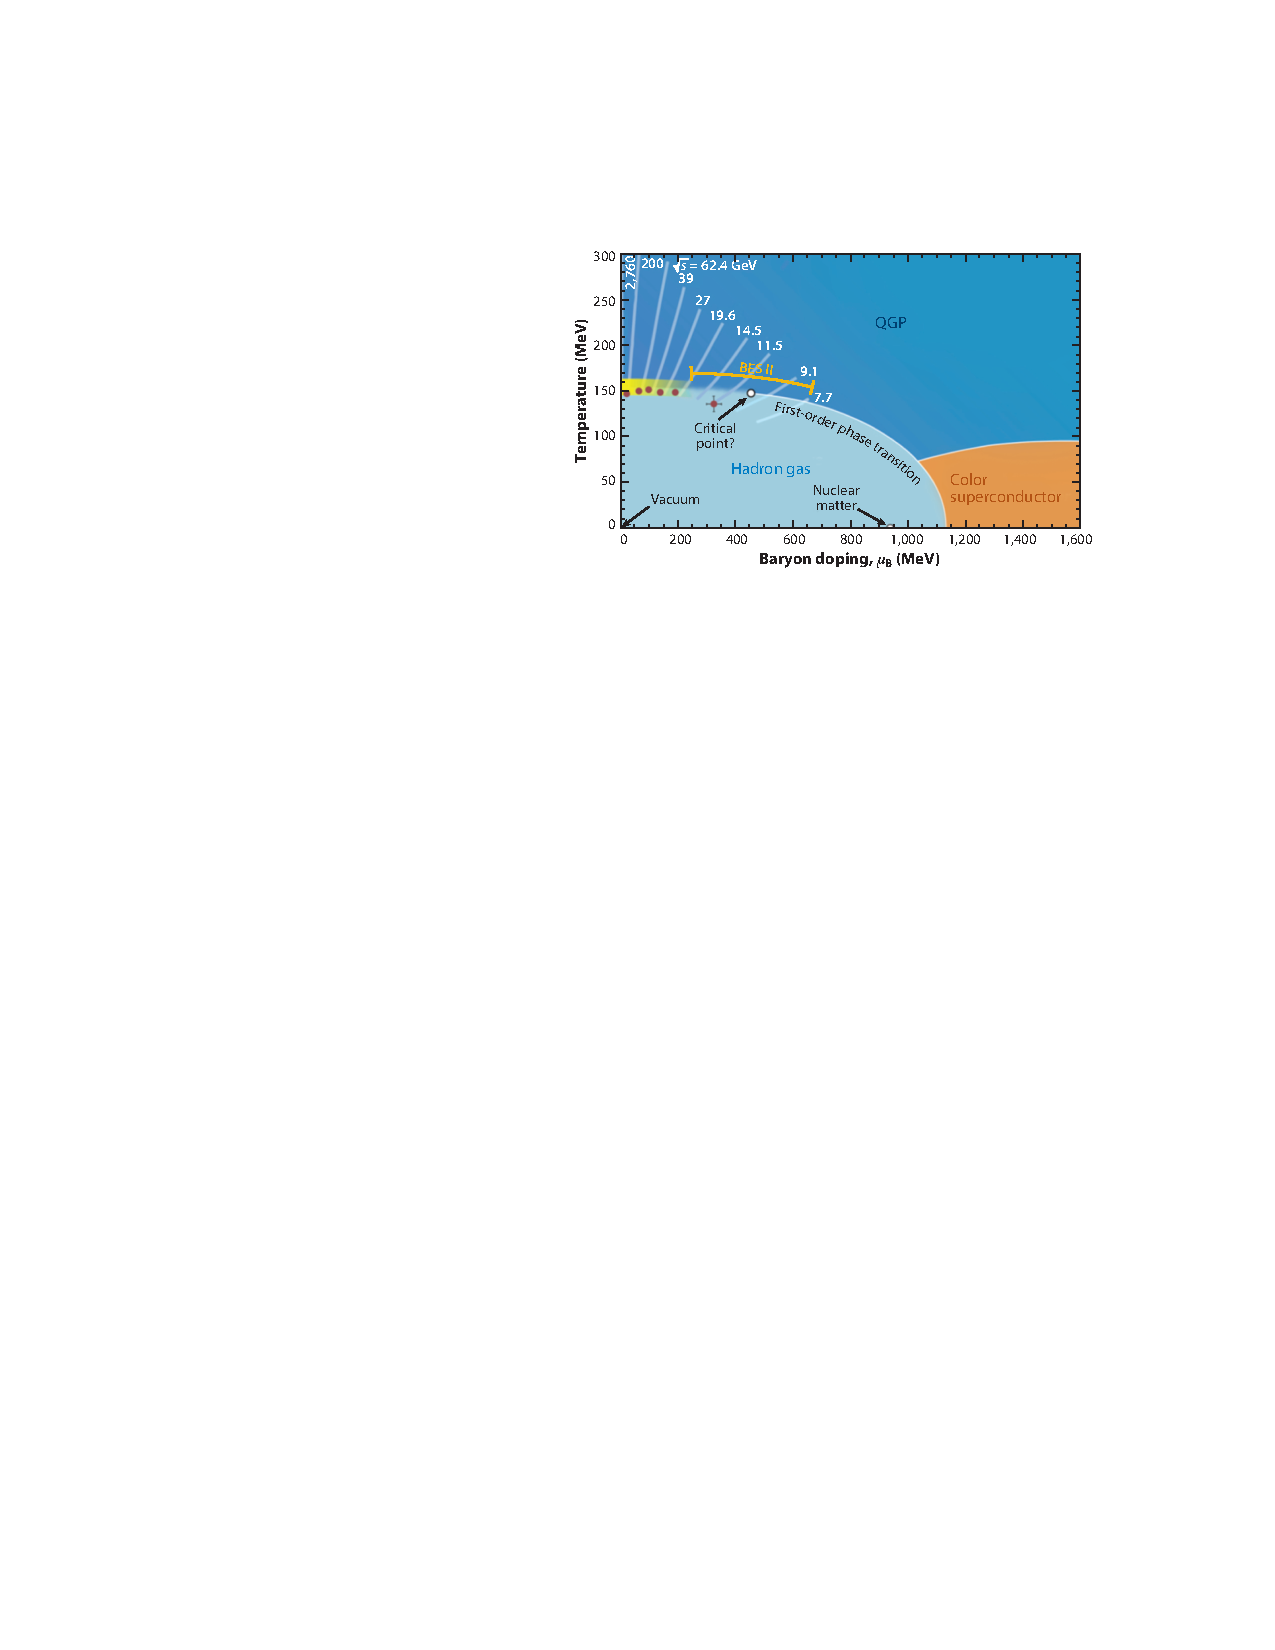
\includegraphics[width=.99\textwidth]{Introduction/qcd_phase.pdf}
  \caption{The current understanding of the expected features of the phase diagram of QCD as a function of temperature and baryon doping \cite{annurev-nucl}.}
\label{fig:qcd_phase}
\end{figure}

At extremely high density and pressure, conditions achieved in relativistic heavy ion collisions, quarks and gluons are no longer bound within hadrons,are characterized by astate of \textit{deconfinement}. The maximum energy density occurs as the two highly Lorentz-contracted nuclei collide. This system is of course not in equilibrium instantaneously, and the large energy density is a consequence of the Lorentz contraction of the lead nuclei. In PbPb collisions, equilibrium is predicted to occur at approximately around 1fm/$c$, where the energy density is 12GeV/fm$^3$, about 20 times the energy density of hadron at 500MeV/fm$^3$. While the temperature of the QGP varies by collision system and energy, it is thought that QGP formed at RHIC in AuAu collisions reaches temperatures of 300MeV, with the higher temperatures obtained in PbPb collisions at the LHC. It becomes clear that the quarks and gluons produced in the collision cannot be described as a system of distinct hadrons. That is not to say, however, the quarks and gluons in this high-energy-density matter are far from independent. After production, the QGP expands until the energy density of the plasma drops below that within an individual hadron and the fluid falls apart into a mist of hadrons (known as "chemical freeze-out"). These hadrons then scatter off one another a few times until they propagate freely in a process known as "kinetic freeze-out".

While the prediction of a QGP state is based on perturbative ideas, its properties cannot be estimated perturbatively. Enter lattice QCD. In the 1970's, a method was discovered where QCD may be calculated computationally at large scales by replacing continuous space with a finite lattice~\cite{Wilson1974}. Lattice QCD is a non-perturbative approach to solving QCD, and when the size of the lattice is taken infinitely large and its sites infinitesimally close to each other, the continuum QCD is recovered. Fig \ref{fig:lattice_qcd} shows lattice QCD calculations for the  pressure p, energy density $\epsilon$, and entropy density s of hot QCD matter in thermal equilibrium at temperature T. Lattice QCD gives several powerful insights on the order of the phase transition from hadronic matter to a quark gluon plasma, the critical temperature at which the phase transition occurs, approximately $T_C\approx$200MeV, as well as the bulk properties of the system shown in Fig.~\ref{fig:lattice_qcd}. Lattice QCD has strict limitations, however. Aside from requiring huge amounts of high performance computing, lattice calculations are built upon the Euclidean formulation of equilibrium thermodynamics, and so it is much more challenging to use them to gain information about transport coefficients such as the shear and bulk viscosities, and it seems very unlikely they can even be used to describe time-dependent processes of the plasma.


\begin{figure}[htpb]
  \centering
  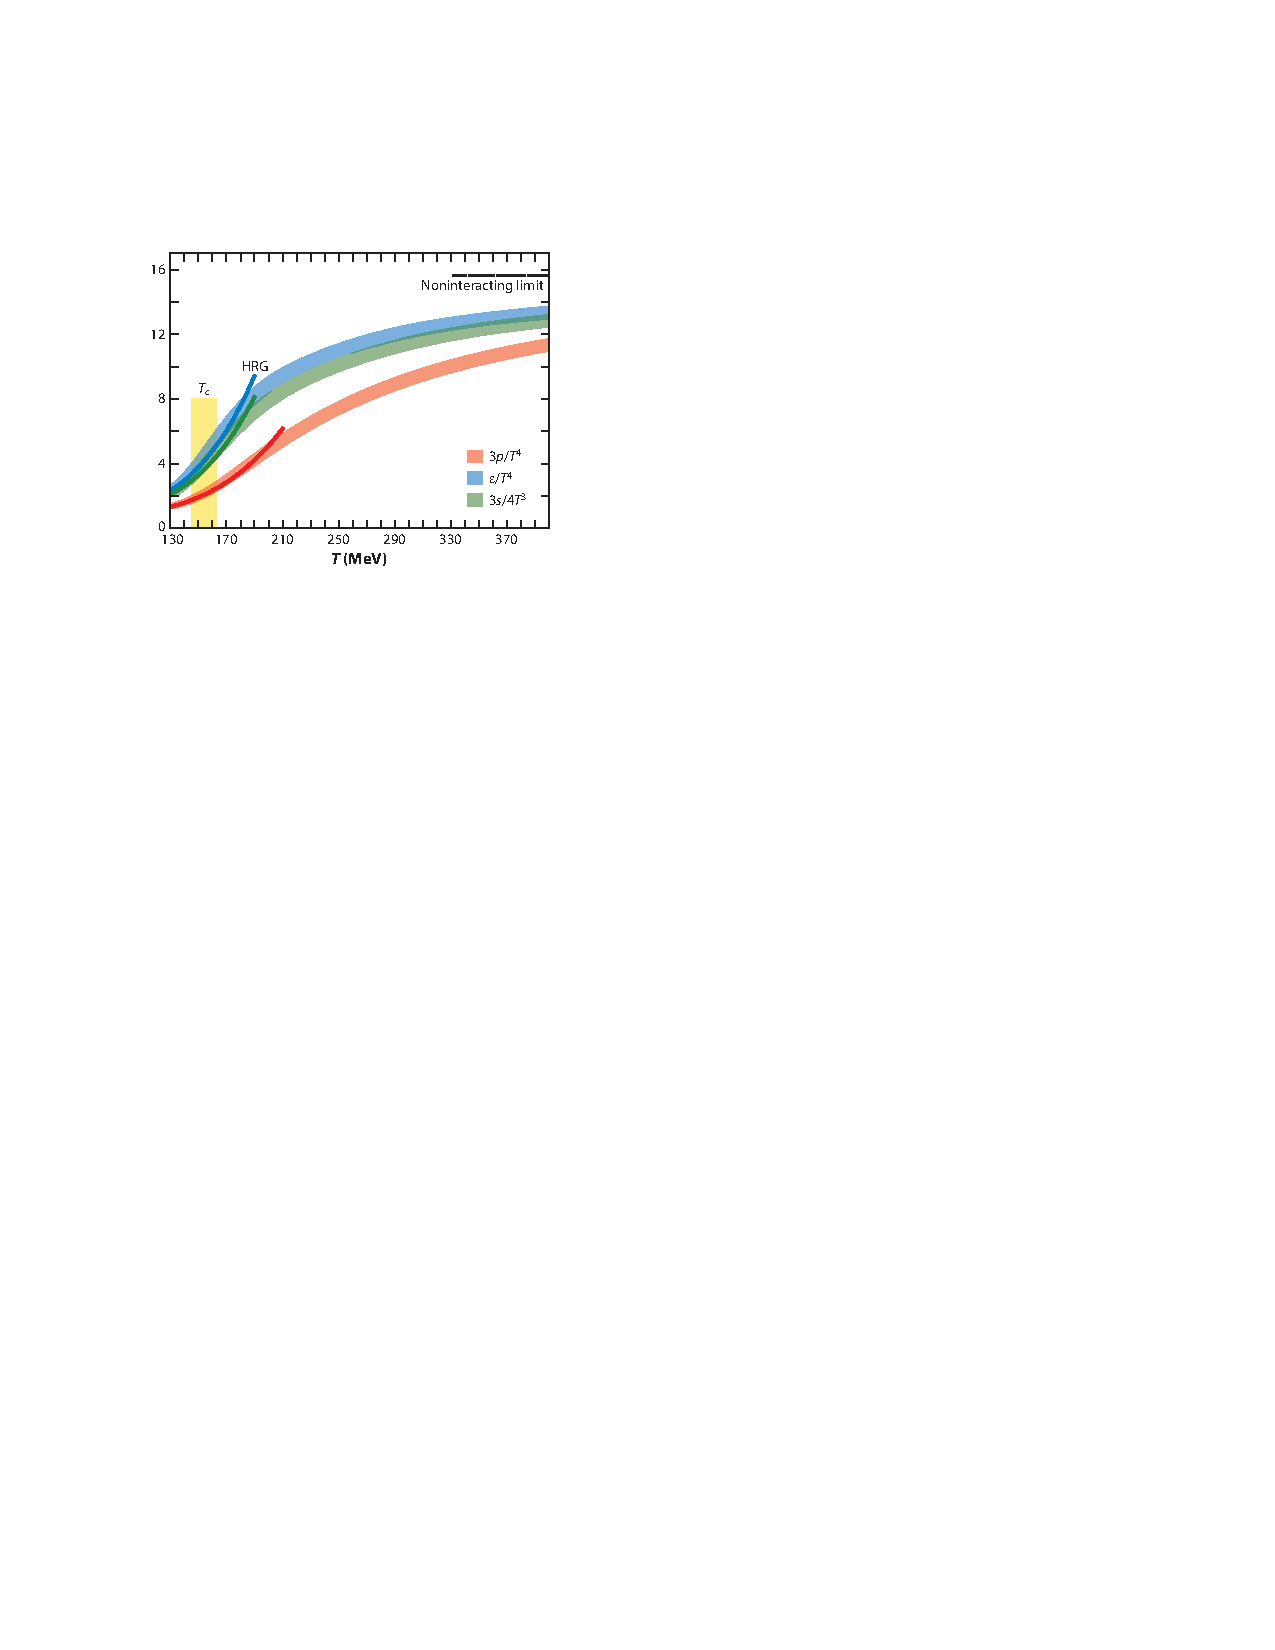
\includegraphics[width=0.8\textwidth]{Introduction/lattice_qcd.pdf}
  \caption{Lattice QCD calculations (colored bands) of the pressure p, energy density $\epsilon$, and entropy density s of hot QCD matter in thermal equilibrium at temperature T \cite{Borsanyi2014,HotQCDCollaboration2014} show a continuous crossover around T$\approx$150 MeV, from a hadron resonance gas (HRG; colored lines) at lower temperatures to quark–gluon plasma (QGP) at higher temperatures, at higher temperatures, a first-order phase transition is expected, as indicated in figure \ref{fig:qcd_phase}\cite{annurev-nucl}.}
  \label{fig:lattice_qcd}
\end{figure}


While Perturbative QCD (pQCD) and lattice QCD calculations have their limitations, in conjunction with the discovery of asymptotic freedom, they all point towards the formation of a state of matter made up of deconfined quarks and gluons. In the next section, experimental evidence of the creation of such a state of matter will be discussed. 

\subsection{Flow}\label{sec:flow}

The original extension of asymptotic freedom predicted that the deconfined state of quark and gluons at high energy densities would behave as an ideal gas. The interplay between two key features of QCD determines the nature of this state of matter. First, because of asymptotic freedom and the high energies probed at RHIC and the LHC, it could be that the interactions between the partons are so weak that the system may never reach thermal equilibrium. Second, at energy scales within an order of magnitude of the confinement/deconfinement energy scale, QCD is strongly coupled. It has only recently been realized after the experiments at RHIC that in this temperature range QCD describes a relativistic fluid consisting of quarks and gluons that are so strongly coupled to each other that the resulting liquid cannot be described in terms of a gas of quasiparticles \cite{Adams2005a}. The weak coupling picture must be correct during the initial stages of the collisions with exceedingly high energy; yet even in these collisions, the strong coupling picture would become applicable at later times, after a hydrodynamic fluid has formed. The timelength of the initial moments of the collisions at RHIC or the LHC where the weakly coupled picture can be applied remains an open question.
%The v2 in small systems also brings into questions the equilibrium timescale to reach equilibrium, and has also spawned a new set of questions on pre-equilibrium hydrodynamics \cite{Romatschke2018}

% On the other hand, if the quarks and gluons form a strongy coupled liquid relatively quickly, the fluid will expand hydrodynamically, where hydrodynamics will convert initial spatial anisotropies to into momentum anisotropies.

As the colliding nuclei do not hit directly head on, there is a non-symmetric overlap region of the two nuclei. This is shown in Fig.~\ref{fig:overlap}, where the cartoon shows the resulting elliptically shaped overlap region produced when two spherical nuclei are involved in a more peripheral collision. This causes a pressure gradient which in turn causes more particles to flow along the direction of the reaction plane, the plane defined by the beam direction and impact parameter (vector connecting the centers of the two nuclei), shown as the green grid in Fig.~\ref{fig:overlap}.

\begin{figure}[htpb]
  \centering
  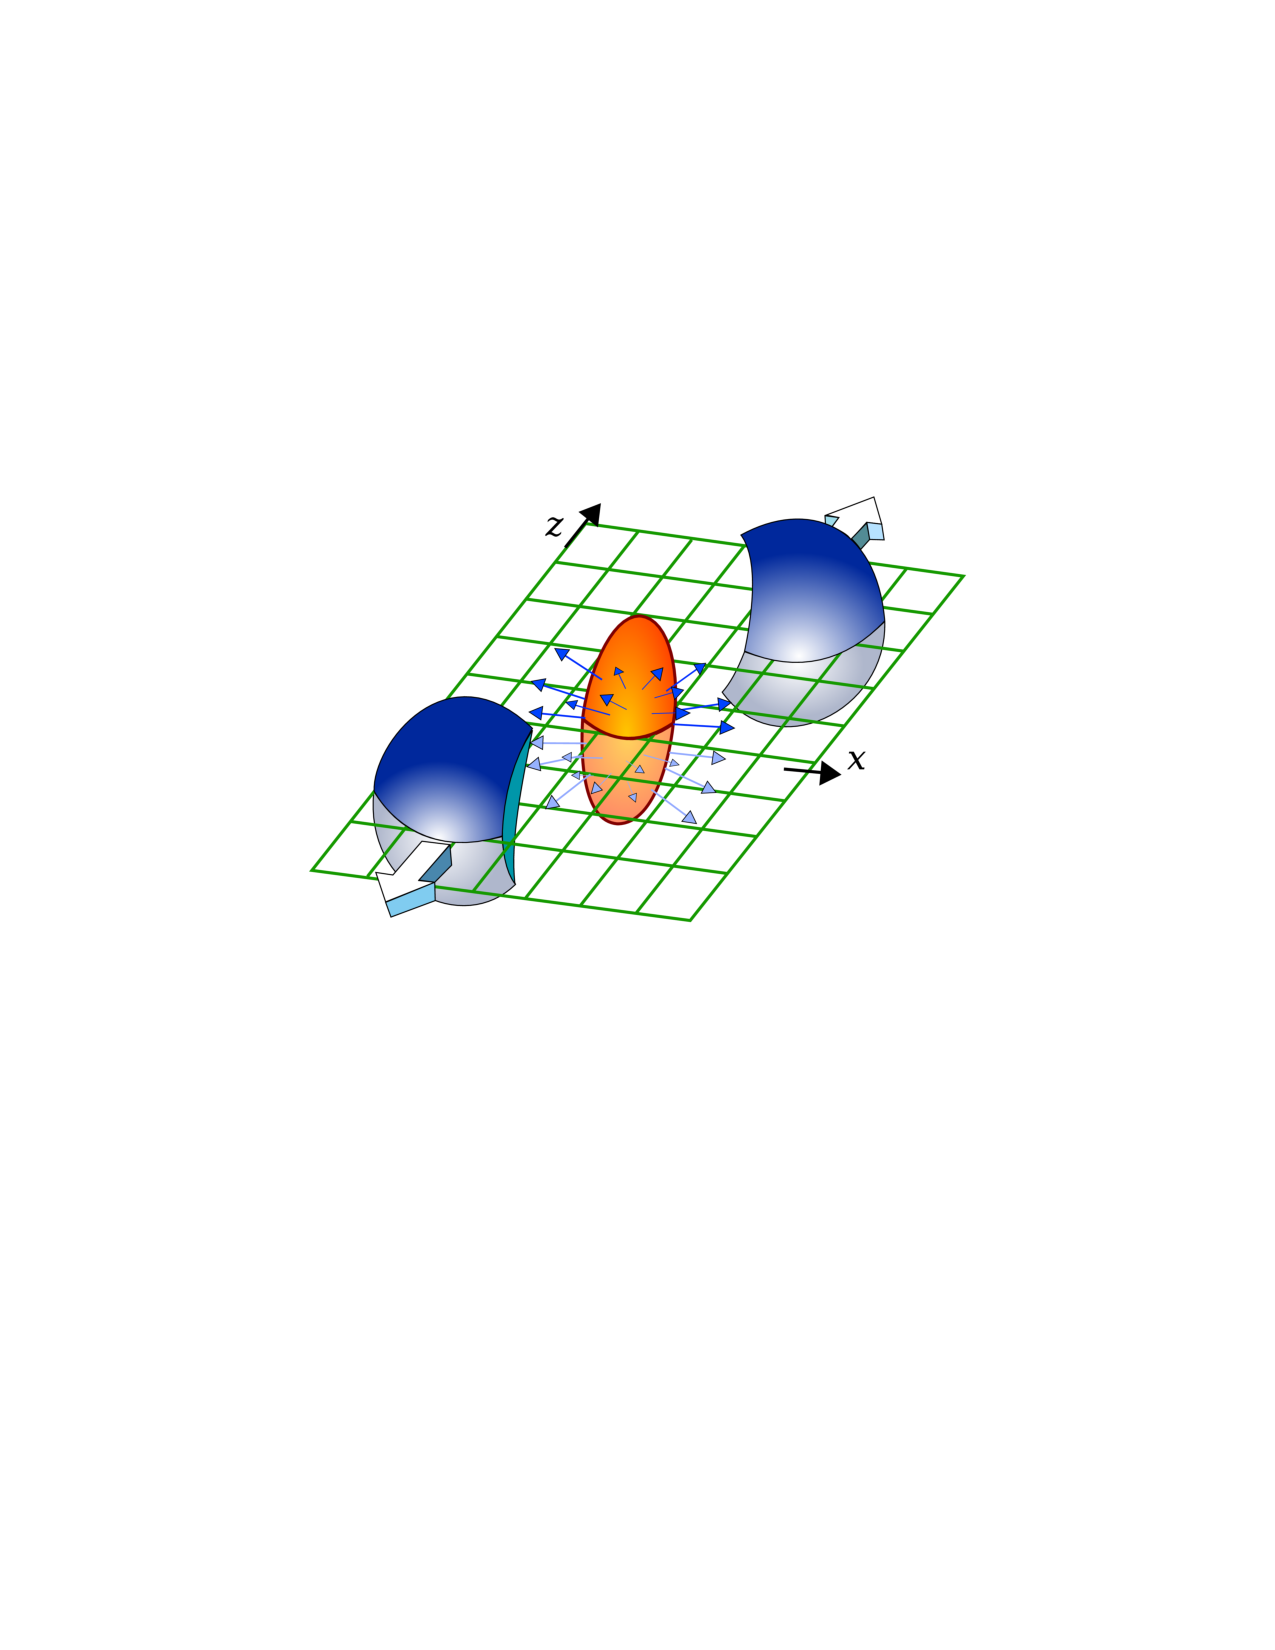
\includegraphics[width=0.8\textwidth]{Introduction/overlap_diagram.pdf}
  \caption{The reaction plane of the collision is shown here for a collision in which the overlap region has an almond-like shape. This spatial anisotropy in the initial collisions results in a flow of particles in the direction of the reaction plane. The reaction plane is defined by the direction of the beams, $z$, and the impact parameter which connects the centers of the colliding nuclei and happens to be along the $x$ direction in this plot.}
  \label{fig:overlap}
\end{figure}

By measuring the anisotropy of particles produced in heavy ion collisions, the crucial distinction between these two scenarios can be found: In the case of a weakly interacting gas of particles, the initial spatial anisotropy of the collision zone would essentially be washed out by random motion, leaving the azimuthal distribution of final state particles roughly isotropic. Alternatively, if the quarks and gluons form a strongly coupled liquid soon enough, while the distribution of energy density produced in the collision remains anisotropic, this noncircular and lumpy drop of fluid will expand in a hydrodynamic fashion, yielding faster expansion in the direction of larger gradients: Hydrodynamics converts spatial anisotropies into momentum anisotropy.

A Fourier transformation is performed to related the measured angular distribution of final state (charged) particles to the azimuthal momentum anisotropy. 

  \begin{equation}
    \frac{\mathrm{d}\bar{N}}{\mathrm{d}\varphi} = \frac{\mathrm{d}\bar{N}}{2\pi} \left(1 + 2\sum^\infty_{n=1}\bar{v}_n\cos[n(\varphi - \bar\Psi_n)]\right)
  \end{equation}

  With $\varphi$ as the angle in the transverse plane, or azimuthal angle, $\bar\Psi_n$ are the event plane angles determined with respect to the beam direction, and $\bar{N}$ is simply the average number of particles of interest in the event. Importantly, $\frac{\mathrm{d}\bar{N}}{\mathrm{d}\varphi}$ is the quantity that is directly measured, and $v_n$ is extracted as a fourier coefficient that quantifies the magnitude of flow. The subscript $n$ indicates the order of the harmonic, with $v_n$ indicating the kind of flow and are thus called \textit{flow coefficients}. For example, $v_1$ corresponds to radial flow, and perhaps more interestingly, $v_2$ corresponds to elliptic flow that results from the initial elliptic overlap region shown in Fig~\ref{fig:overlap}. $v_2$ has been measured extensively at RHIC and the LHC, and has been showed to be non-zero and positive. This strongly indicates that the picture of a strongly coupled fluid that is formed proceeding the initial collision is the correct picture.  

  This cartoon is of course a simplification: the nuclei are made up of nucleons (in tern made of partons) and are quite lumpy, resulting in more complex spatial anisotropies in the initial collision, and therefore higher order flow coefficients. The interacting nucleons and partons of the initial collision give rise to different collision geometries, which can result in non-zero measurements of higher order flow harmonics. This is demonstrated beautifully in Fig~\ref{fig:collision_geometries}, where different nuclei of distinct shapes, $^3$He, deuterium, and protons, are simulated to completely collide with Au to observe simple yet very distinct collision geometries \cite{Aidala2019}. 
  
  \begin{figure}[htpb]
    \centering
    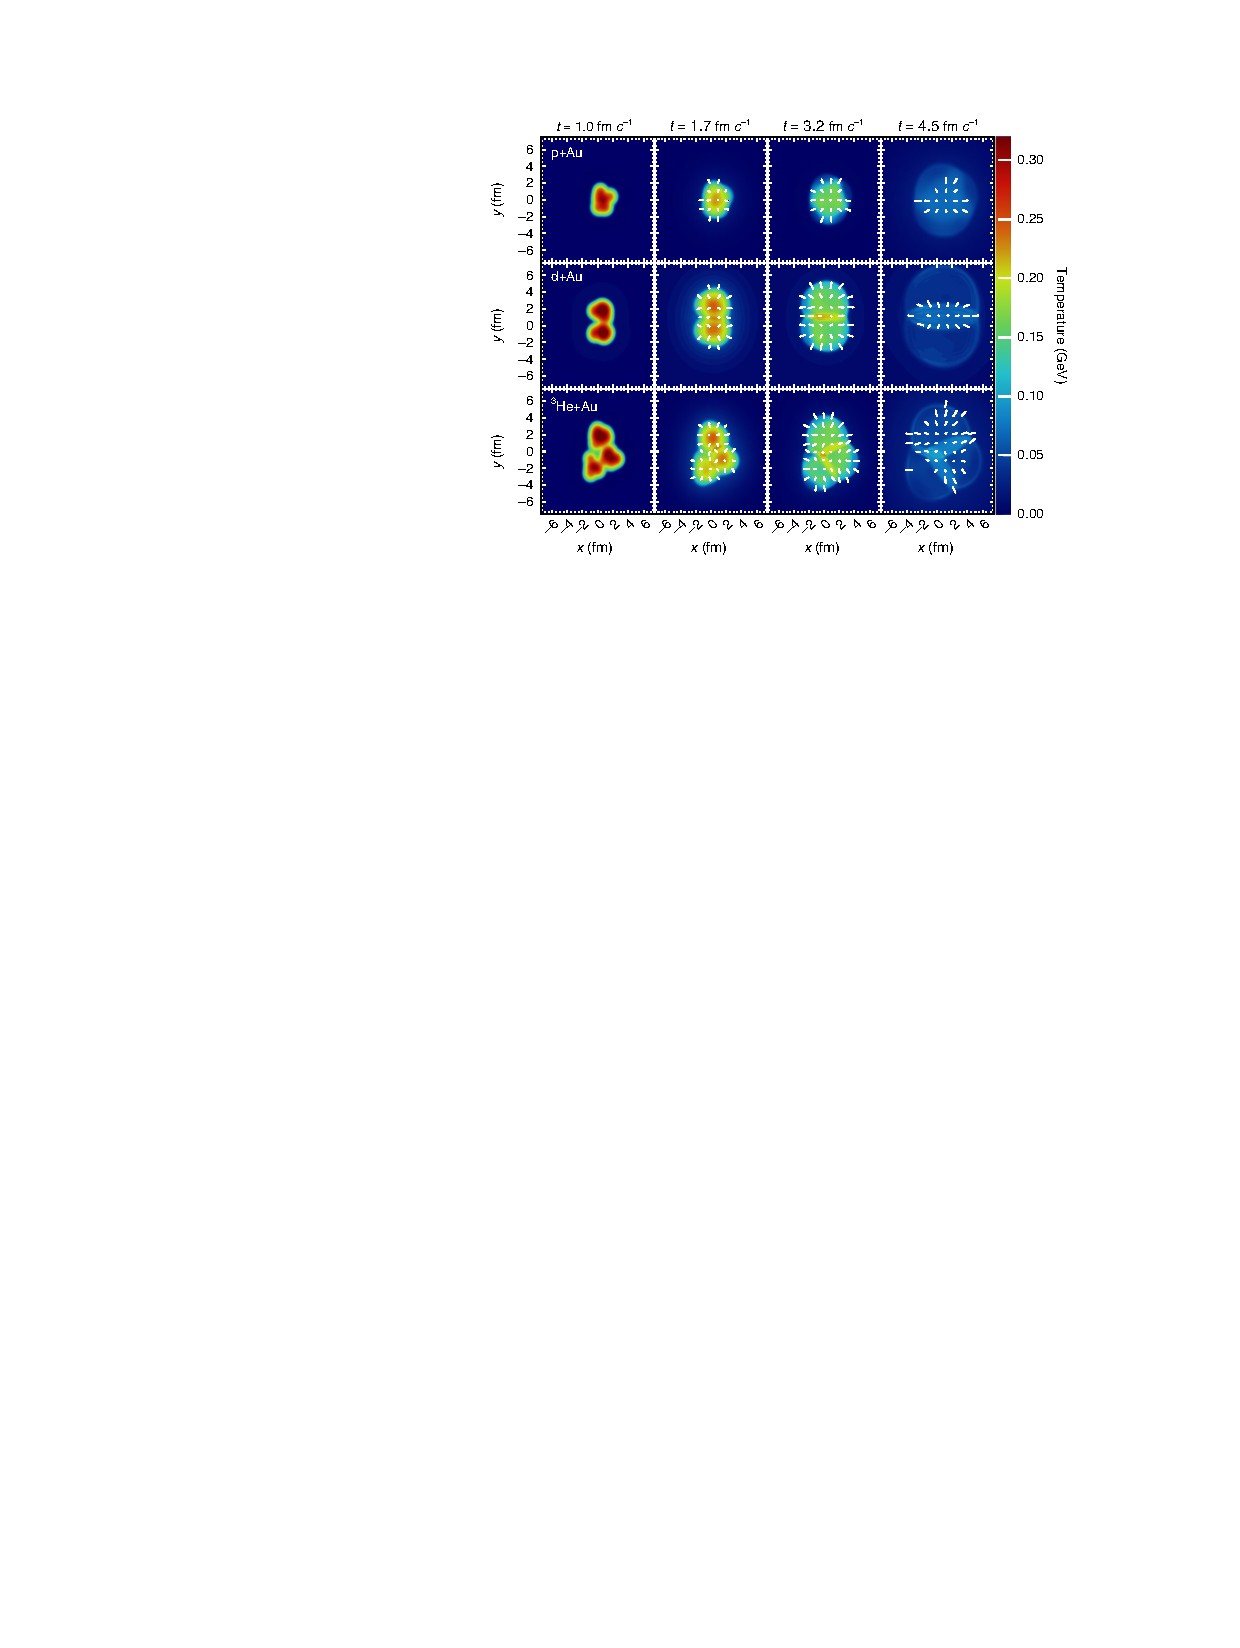
\includegraphics[width=0.8\textwidth]{Introduction/collision_geometries.pdf}
    \caption{Hydrodynamic evolution of a typical head-on p+Au (top), d+Au (middle) and $^3$He+Au (bottom) collision at $\sqrt{s_\mathrm{NN}}$ = 200 GeV as calculated by SONIC, where the p/d/3He completely overlaps with the Au nucleus. From left to right each row gives the temperature distribution of the nuclear matter at four time points following the initial collision at t = 0. The arrows depict the velocity field}
    \label{fig:collision_geometries}
  \end{figure}

  The bottom most panel would correspond to an larger $v_3$ measurement. Higher flow harmonics larger systems (AA and PbPb) have been measured as well. Fig \ref{fig:flow_measurements} shows such measurements up to $v_5$ \cite{Aamodt2011}. 

  \begin{figure}[htpb]
    \centering
    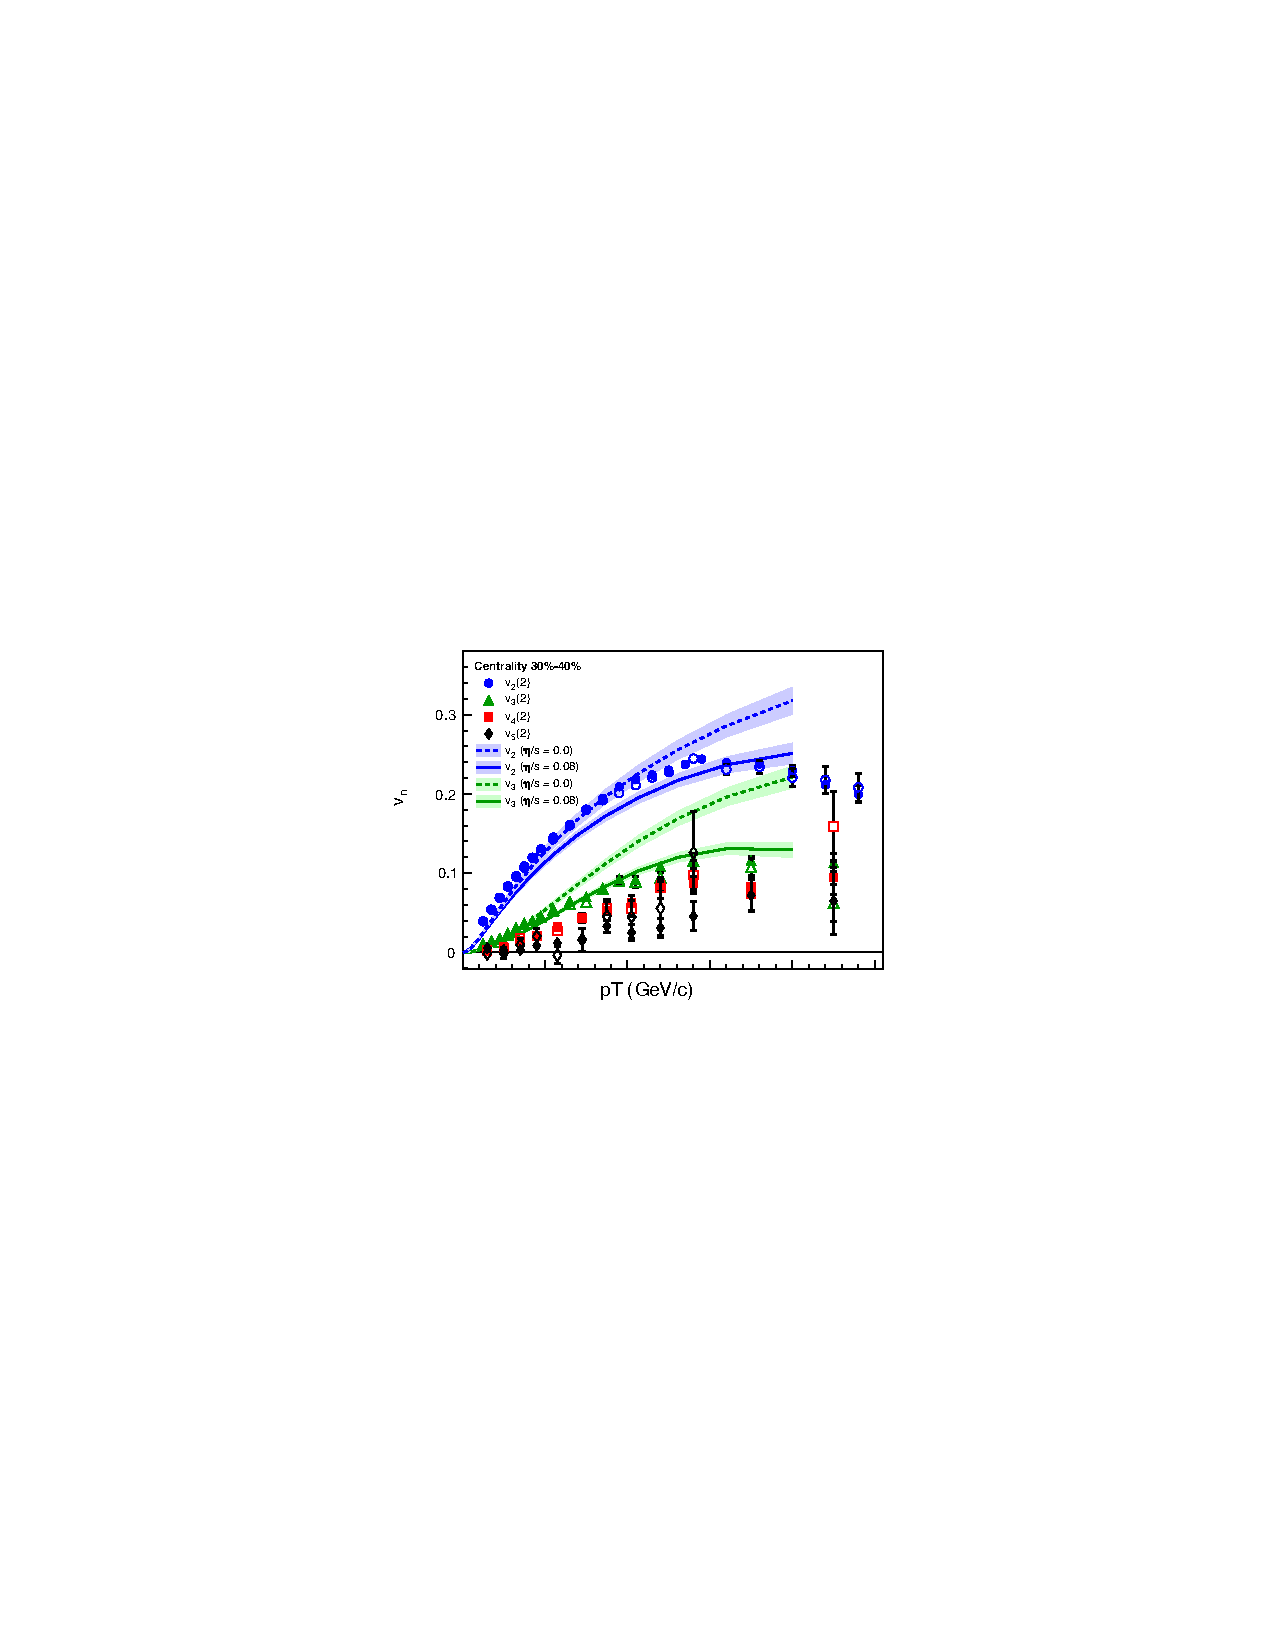
\includegraphics[width=0.45\textwidth]{Introduction/flow_measurements_peripheral.pdf}
    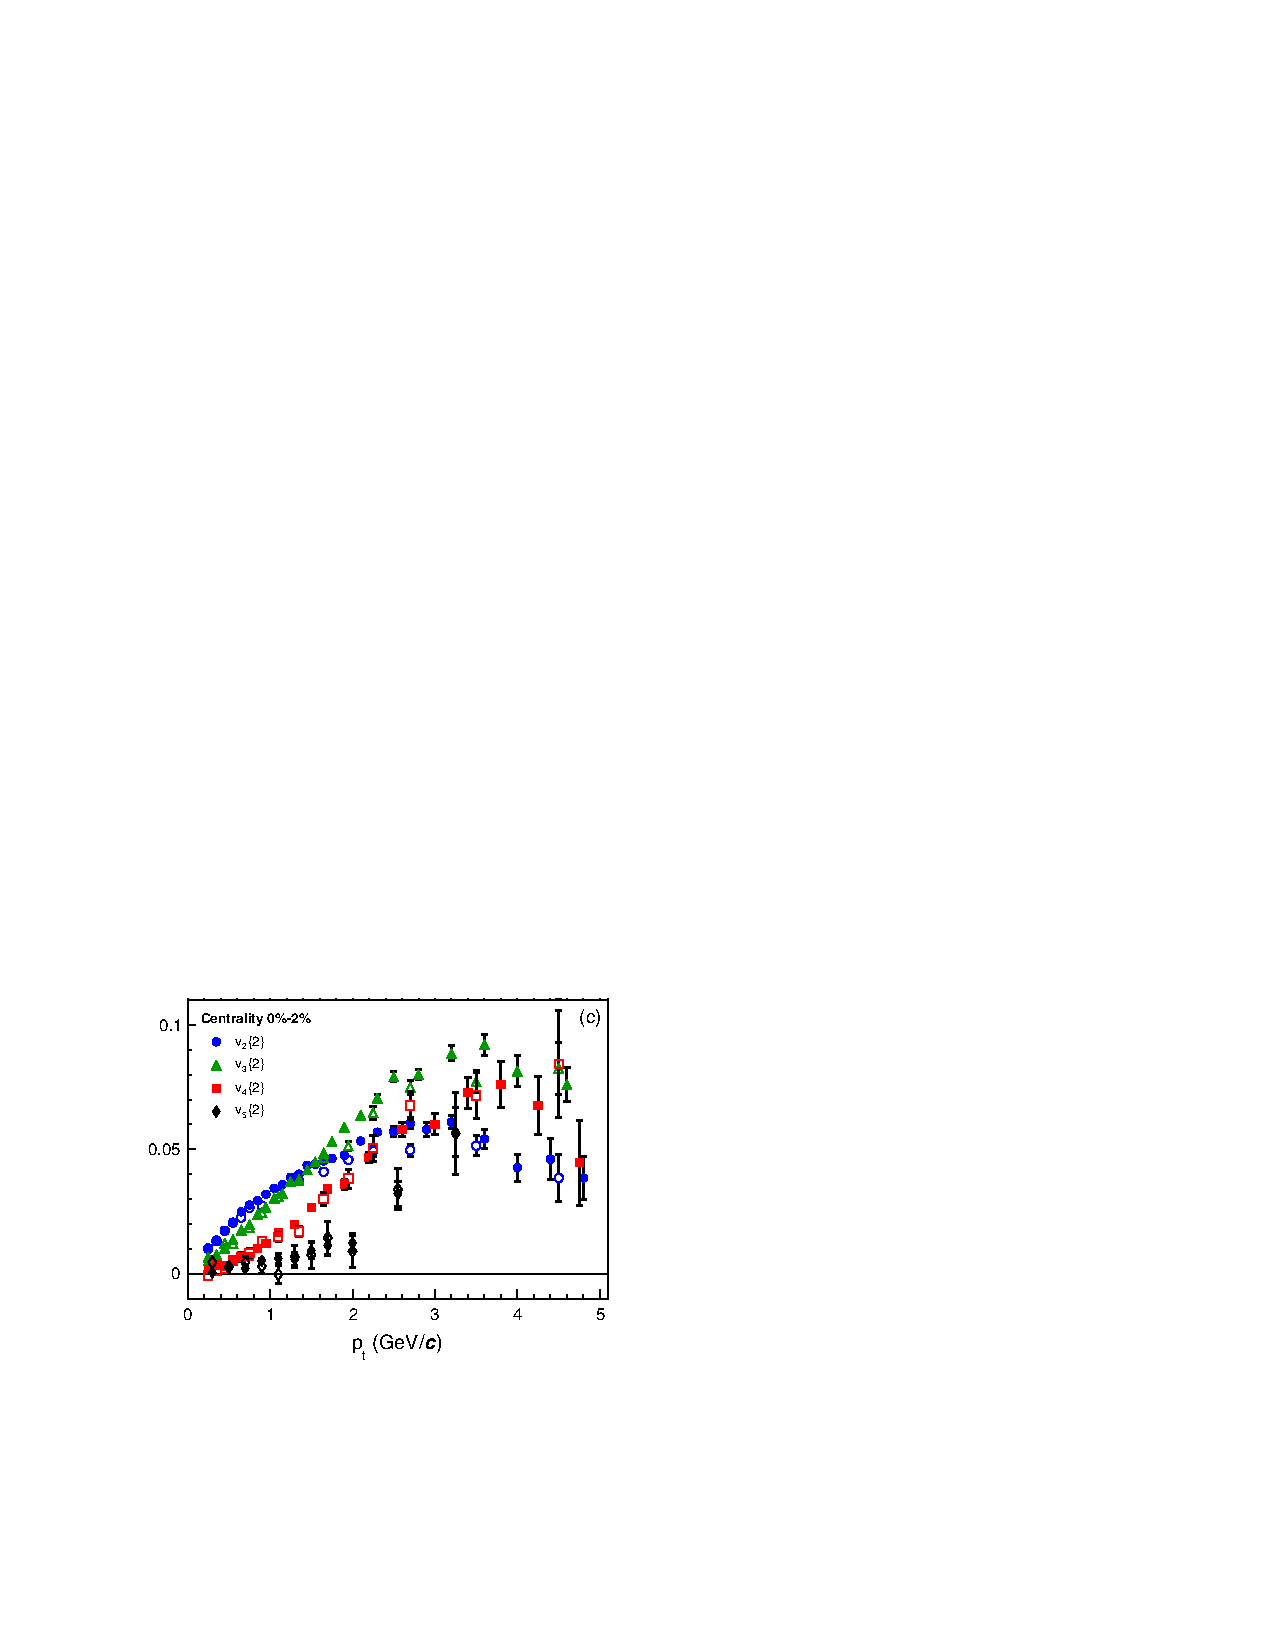
\includegraphics[width=0.45\textwidth]{Introduction/flow_measurements_central.pdf}
    \caption{$v_2, v_3, v_4$, and  $v_5$ as a function of transverse momentum for peripheral (left) and central (right) PbPb events. The full and open markers are for  $\Delta\eta < 0.2$ and  $\Delta\eta < 1.0$, respectively. The colored bands represent hydrodynamic models with two different parameters for the specific viscosity.}
    \label{fig:flow_measurements}
  \end{figure}


  The property that quantifies the liquidness of a material made up of ultrarelativistic constituents is the ratio of its shear viscosity $\eta$ to entropy density, $s$. The ratio $\eta/s$ is dimensionless in units where $k_B$ and $\bar{h}$ have been set to 1. This ratio plays a key role in the equations of hydrodynamics which govern the effects of shear viscosity in a relativistic fluid, and is often called the ''specific viscosity''. The precise magnitude of the anisotropies $v_n$ should then be quite sensitive to the viscosity of the plasma. Specific viscosity controls how rapidly gradients of any sort introduced in the initial conditions are dissipated into heat. This means that flow measurements compared to theory calculations can constrain the specific viscosity. By using simulations with smooth initial conditions (obtained from lattice calculations),  it can be estimated that the specific viscosity of the QGP is approximately 0.08-0.20 \cite{Romatschke2007}. The lower end of which is remarkably close to the theoretical limit for any liquid of 1/$4\pi$. For this reason, the quark gluon plasma is often called the most perfect liquid.

 % meaning that it is this quantity which is ultimately constrained by comparing hydrodynamic calculations with data
 % Alternatively, if the quarks and gluons form a strongly coupled liquid soon enough, while the distribution of energy density produced in the collision remains anisotropic, this noncircular and lumpy drop of fluid will expand in a hydrodynamic fashion, yielding faster expansion in the direction of larger gradients: Hydrodynamics converts spatial anisotropies into momentum anisotropy

% Specific viscosity controls how rapidly gradients of any sort introduced in the initial conditions are dissipated into heat, meaning that it is this quantity is ultimately constrained by comparing hydrodynamic calculations with data.


\subsection{Flow in Small Systems}
It should be noted, however, that flow -- a key signature of a viscous fluid -- is not exclusive to AA collisions. Non-zero measurements of flow have been observed in high multiplicity pp collisions at CMS \cite{Khachatryan2010} and in p--Pb collisions at ALICE and LHCb \cite{Abelev2013,Aaij2016} . Figure \ref{fig:near_side_ridge} shows the famous "near side ridge" in high centrality p--Pb, a feature most likely attributable to the hydrodynamic evolution of the initial collision geometry (closely related to $v_2$).

\begin{figure}[htpb]
  \centering
  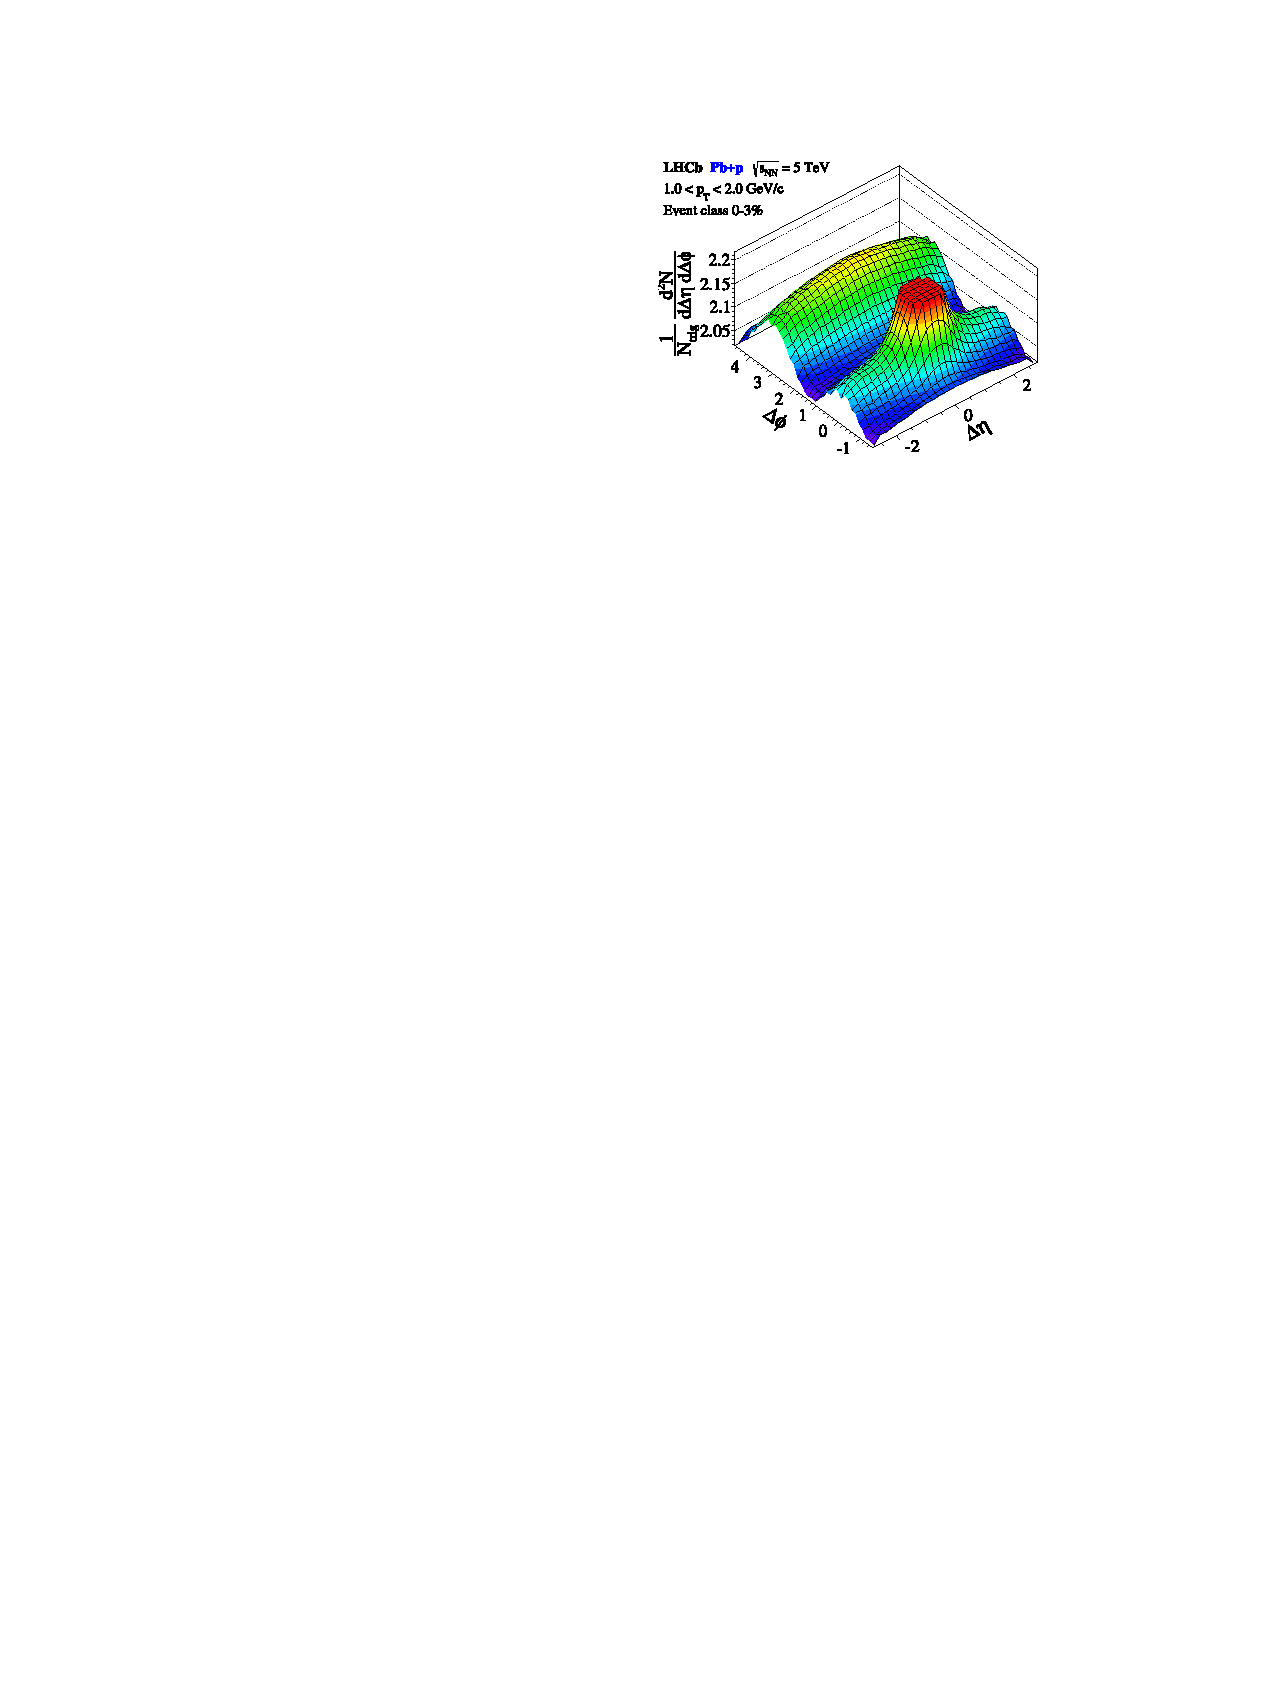
\includegraphics[width=0.8\textwidth]{Introduction/near_side_ridge.pdf}
  \caption{Two-particle correlation for high-event activity in p–Pb collisions at 5.02 TeV measured with the LHCb detector \cite{Aaij2016}.}
  \label{fig:near_side_ridge}
\end{figure}

\kt~smearing is responsible for the away side jet peak being broader than the nears side jet peak. This is because in the simple 2-2 scattering picture in which the initial total pt is 0, the two scattered partons should be back-to-back in \deltaphi~to conserve momentum. However, the partons in the initial system  do not \textit{necessarily} have 0 \pT. Both partons can have an initial transverse momentum, \kt, that makes up a component of their overall momentum fraction of the nucleon, bjorken-x. The ''near-side ridge'' observed here is often thought to be the result of collectivity or flow, hinting that there there may be some hydrodynamic behavior even in these small systems. The degree of hydrodynamic behavior can be quantified by $v_2$, as mentioned before, and is shown in Fig.~\ref{fig:small_systems_v2}, where a non-zero  $v_2$ in pp, and p--Pb (as well as PbPb) is shown:
% Figure \ref{fig:small_systems_v2} shows the measured, non-zero $v_2$  in pp, p--Pb and PbPb. 
\begin{figure}[htpb]
  \centering
  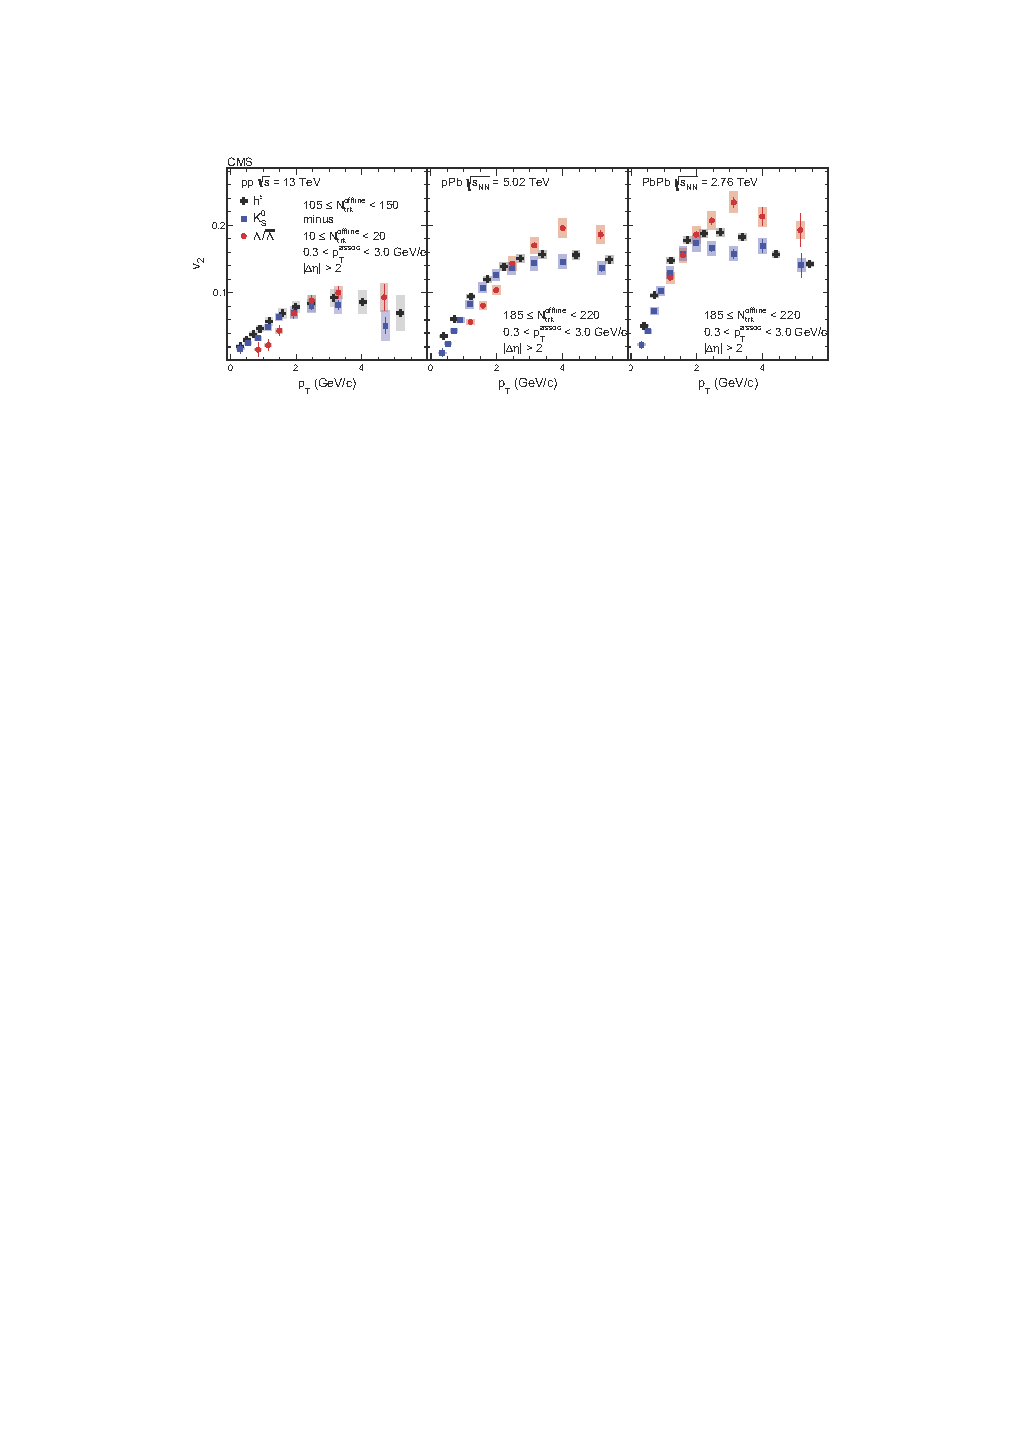
\includegraphics[width=0.99\textwidth]{Introduction/small_systems_flow.pdf}
  \caption{The $v_2$ data measured in pp, pPb and PbPb collisions by CMS as a function of $p_\mathrm{T}$ for charged particles, $K_0^s$ and $\Lambda$ particles at high multiplicities from two-particle correlations \cite{Khachatryan2017,Khachatryan2015}.}
  \label{fig:small_systems_v2}
\end{figure}

These observations came as quite the surprise: These smaller systems were previously thought to have insufficient energy density for deconfinement to occur and contained too few particles in the collision for thermalization and the equations of hydrodynamics to meaningfully apply.

% The observation of the near side ridge as  well as non-zero $v_2$ (both observed in pp and p--Pb) has called into question the assumption that QGP is not produced in these smaller systems. Additionally, the case of pp is particularly interesting, as the number of particles was also thought to be too small to meaningfully reach a state of thermalization, nor to be reasonably described by hydrodynamics. This has spawned quite interesting work on the applicability of hydrodynamics in systems far from equilibrium \cite{Romatschke2018a}.

The observation of flow, however, is not a sufficient condition to for claiming the creation of quark gluon plasma. One hypothesis claims that this phenomenon is not solely attributable to the formation of QGP. Recently there has been quite interesting work on the applicability of hydrodynamics in systems far from equilibrium \cite{Romatschke2018a}, and findings that indicate that measurements of $v_n$ do not necessarily imply equilibrium \cite{Romatschke2017}. But the question of why hydrodynamics describes these small systems so well \cite{Habich2016, Zhao2018a} remains an open question in the field \footnote{One should be careful to mention that hydrodynamics do not exclusively reproduce}. On the other hand, another hypothesis is that a tiny droplet of QGP is formed in these smaller systems. While our current understanding of the conditions required for the formation of QGP indicates that it may in fact be possible to create a QGP in these systems, this is troubling for other reasons. These smaller systems often serve a "control" for quantifying the modifications observed in AA collisions that are attributed to QGP. This all points to the increased necessity of measuring modifications in smaller systems, particularly attempting to disentangle the effects of hot nuclear matter from cold nuclear matter, and is a principle focus of this thesis.

As stated previously, the presence of flow effects in small systems has not unambiguously stipulated the creation of a quark gluon plasma in these systems.  Other observables such as the broadening of the away side correlation, and enhanced strangeness production need to be studied. In particular, however, a "smoking gun" of QGP production, discussed in the next section, has yet to be observed in small systems, despite an extensive search for it.


\subsection{Jets}
The next key piece of evidence for the production of a hot, deconfined nuclear matter has to do with the observed modification of jet production in heavy ion collision. But before discussing this observable, it will be useful to discuss exactly what a jet is, and perhaps more fundamentally, how partonic interactions are related to experimental observables such as the data in Fig.~\ref{fig:a_S_running}. Generally, the perturbative regime of QCD is explored using high energy collisions of elementary particles, the simplest of which are electron-positron collisions. In these collisions, quarks may be produced in the final state by the reaction $e^++e^- \rightarrow q\bar{q}$. Yet, due to confinement these quarks are not observed at the detector level, but rather hadronize into a collimated spray of mesons and baryons, which are correlated in phase space and collectively referred to as \textit{jets}. 

At a high level, a jet represents a virtual hard parton and its subsequent evolution. In practice, a jet is a 'contract between experimentalists and theorists': hadrons are combined into jets using specific definitions and reconstruction algorithms (most prominently the Anti-$k_\mathrm{T}$ and Cambridge/Aachen algorithms~\cite{Atkin2015}) cleverly based on pCQD arguments. 

\subsection{Nuclear Modification Factor}
\label{sec:raa}
Jet production and showering in vacuum are well described by pQCD, as shown in the blue triangles and green asterisks in Fig.~\ref{fig:a_S_running}. When a jet is produced in a heavy ion collision, however, the partons in the shower must barrel through the droplet of QGP produced in the same collision. As this happens, the jets should loose energy and forward momentum, as the plasma should be opaque to color charge in the same way a more traditional ionized plasma is opaque to light.  Thus a key signature of the formation of a quark gluon plasma in the lab is the observation of this \textit{jet energy loss} or \textit{suppression}. This loss of course, is simply the redistribution of the jets energy to the medium, and must be compared to how jets propagate in 'vacuum' (to which pp collisions is taken as an estimation) in order to be quantified. Accordingly, this suppression is quantified by the nuclear modification factor $R_\mathrm{AA}$. 

  \begin{equation}
    R_\mathrm{AA}(p_\mathrm{T}) = \frac{\mathrm{d}N^\mathrm{AA}/\mathrm{d}p_\mathrm{T}}{\langle N_\mathrm{coll}\rangle\mathrm{d}N^\mathrm{pp}/\mathrm{d}p_\mathrm{T}},
    \label{eq:raa}
  \end{equation}

  where $\mathrm{d}N^{xx}/\mathrm{d}p_\mathrm{T}$ is the number of jets (or, in other contexts, particles of a specified type) produced in AA or pp collision. Additionally, the nuclear modification factor is expressed here as a ratio of yields instead of cross sections \footnote{Other nuclear modifications factors are $T_\mathrm{AA}$, which includes the ratio of cross sections, and $I_\mathrm{AA}$, which is a ratio of conditional yields}. $\langle N_\mathrm{coll}\rangle$ is the total number of encounters between left and right moving nucleons, which we call the number of binary collisions. While $N_\mathrm{coll}$ cannot be determined directly from measured cross sections, there is a well-defined theoretical procedure called a Glauber model calculation \cite{doi:10.1146/annurev.nucl.57.090506.123020} for determining this and other quantities such as the collision impact parameter number of participating nucleons, and centrality classes (percentile classes of multiplicity, or the total number of particles measured in the event). This is applied as an important scaling factor where nuclear collisions are naively modelled to be the sum of many independent p+p collisions. Deviations from this scaling, i.e. a modification factor that deviates from 1, indicate that properties of the nucleus or the creation of a plasma are effecting the measurement.

  $R_\mathrm{AA}$ is the ratio of the observed per-event yield in nuclear collisions to the expected yield. Figure \ref{fig:atlas_raa} shows $R_\mathrm{AA}$ for PbPb collisions.
  \begin{figure}[htpb]
    \centering
    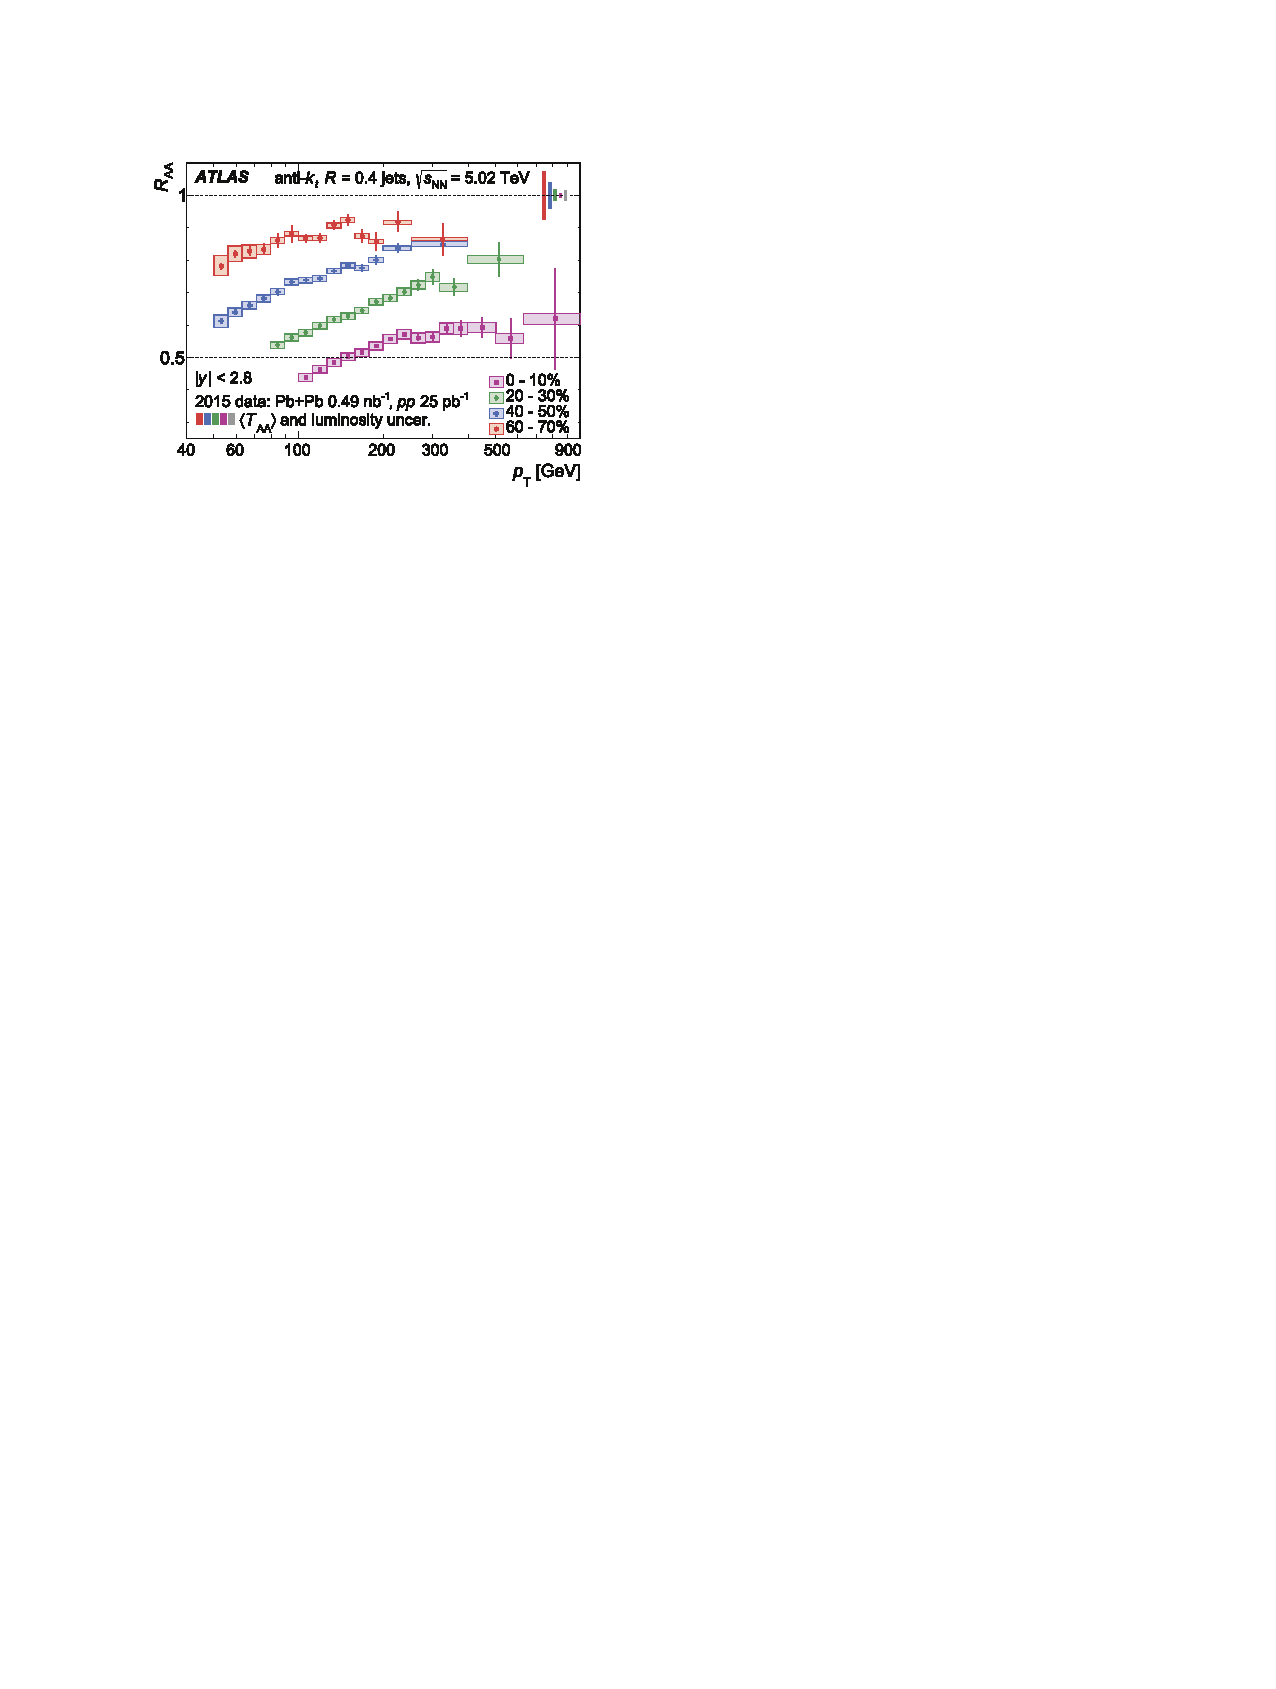
\includegraphics[width=0.8\textwidth]{Introduction/atlas_raa.pdf}
    \caption{The nuclear modification factor $R_\mathrm{AA}$ for jets for four different centralities as a function of jet transverse momentum $p_\mathrm{T}$ \cite{Aaboud2019}. $T_\mathrm{AA} = \langle N_\mathrm{coll}\sigma^{pp}\rangle$}
    \label{fig:atlas_raa}
  \end{figure}
  The amount of suppression shown in Fig.~\ref{fig:atlas_raa} is quite striking, especially for more central events, where the droplet of QGP that the jets need to traverse is largest. This measurement indicates the formation of a medium that is opaque to color charge, and results to the suppression of high \pT~ partons. It is considered an extremely important piece of evidence towards the creation of the quark gluon plasma in relativistic heavy-ion collisions. 

  It is important to realize, however, that high-$p_\mathrm{T}$ jets are produced with a probability that drops rapidly with increasing \pT \cite{Acharya2020}. The steepness of the energy spectrum implies that a small fractional jet energy loss corresponds to a large suppression in $R_\mathrm{AA}$ for jets (this is often referred simply as a ''bin-migration'' effect). This means higher jet \pT~ bins have much lower $R_\mathrm{AA}$ values since each jet that de-populates that bin represents a larger fraction of the total bin count than at lower \pT. In reality, different jets with the same initial energy lose very different amounts of energy, as discussed below, meaning that this argument must be made at the ensemble level. However, the conclusion is the same: the steepness of the jet energy spectrum means the suppression in $R_\mathrm{AA}$ for jets is a very sensitive measure of jet energy loss. 
  % This argument, however, does not apply in the same way for $R_\mathrm{AA}$ measured for single particles.
% The production probability for jets produced at midrapidity scales roughly as $\pT^{-6}$ \ref{annurev-nucl}, for jets with \pT~ values that are not within an order of magnitude of the beam energy.
  The trend for each centrality class is roughly the same, however, where jets at higher \pT~ have modification factors closer to 1. Because of the steepness of the jet spectrum described above, the ensemble of high \pT~ jets that comes out of the droplet of QGP will be dominated by those jets that lost relatively little energy. To put it another way, There are fluctuations in how much energy each individual parton will lose in the medium, and selecting jets which look like high \pt jets in a vacuum may skew measurements towards partons which have lost the least energy in the medium. This is often called the ''survivor bias''~\cite{Connors2018}.

  Fig.~ \ref{fig:raa_particles} shows the $R_\mathrm{AA}$ measured for a variety single particles \cite{Bencedi2016} measure by ALICE and CMS. 

  \begin{figure}[htpb]
    \centering
    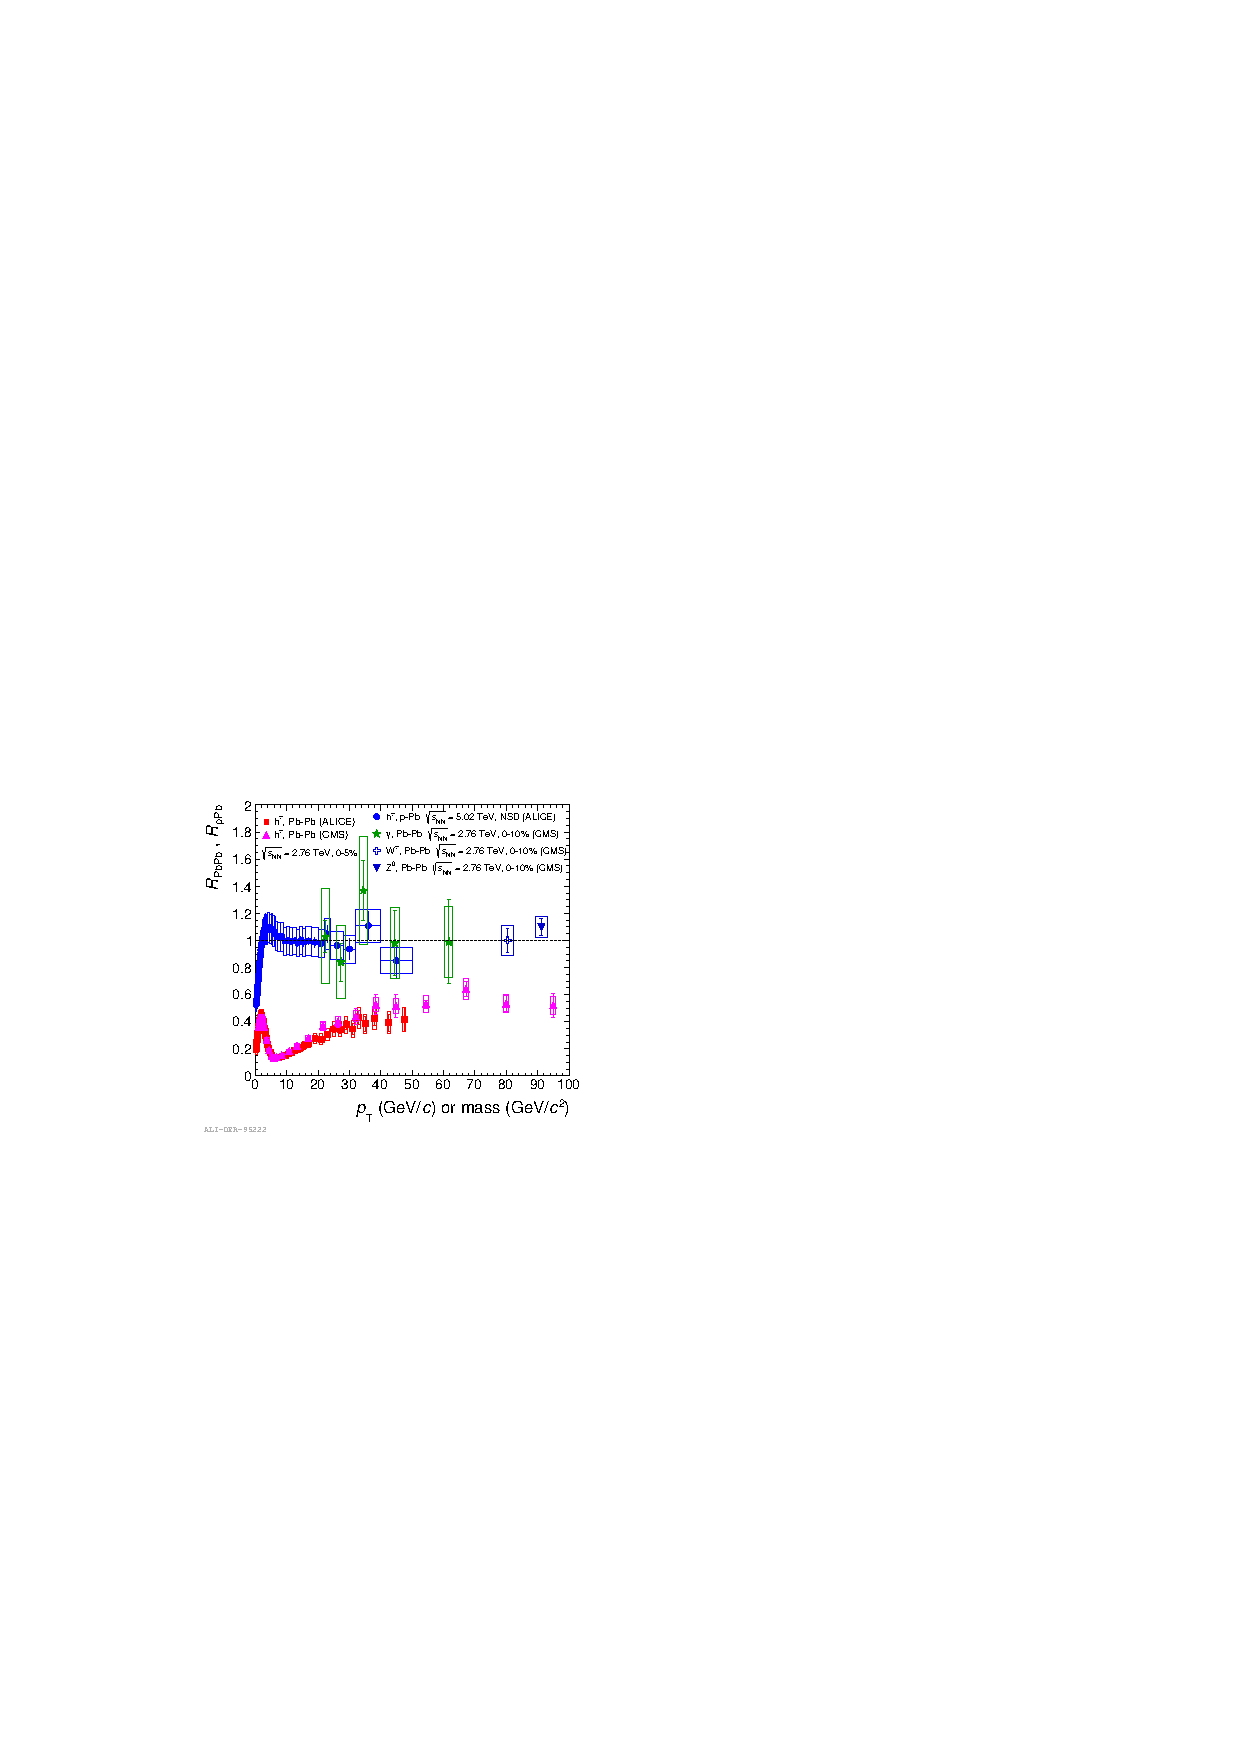
\includegraphics[width=0.99\textwidth]{Introduction/alice_hadron_raa.pdf}
    \caption{Comparisons of $R_\mathrm{PbPb}$ and $R_\mathrm{pPb}$ for various single particles measured by ALICE and CMS \cite{Bencedi2016}.}
    \label{fig:raa_particles}
  \end{figure}

  The single particle $R_\mathrm{AA}$ distributions provides several insights. First, for the bosons measured in the figure, the $R_\mathrm{AA}$ is consistent with unity. This is a vitally important check to validate the definition $R_\mathrm{AA}$ and the scaling of cross sections using Glauber calculations, as these particles are not expected to interact with the medium. This will be discussed in more detail in \ref{sec:direct_photons}. Second, the shape. While an overall suppression is seen, the peak at low \pt~is more likely the result of cold nuclear matter effects, i.e. changes due to the presence of the lead nucleus alone in pPb collisions, instead of hot nuclear matter (QGP). Third, the shape at high \pT. Note that measuring $R_\mathrm{AA}$ for high-\pT~ hadrons is quite different: In both pp and AA collisions, a high-\pT~ hadron is statistically likely to come from a specific, unusual type of jet that contains one very hard parton and is very narrow; Wider jets are intuitively predicted to loose less energy in the medium, and some evidence for this has been observed in \cite{Khachatryan2016}. Selecting (i.e., triggering on) hadrons therefore constitutes selecting an unusual sample of jets that lose less energy, and this selection effect becomes stronger at higher \pT.

  % ThisisonereasonthatRAA for hadrons rises at the highest pT even though RAA for jets remains comparably suppressed

\section{Fragmentation Functions and Factorization of Hard Processes}
\label{sec:FF}
One of the simplest ways to study QCD is to measure the hadronic production in $e^+ + e^-$ collisions, particularly through the process  $e^+ + e^- \rightarrow q\bar{q}$. The inclusive cross section for hadron production ($\sigma$) may be written as the product of the partonic cross section ($\hat{\sigma}$) and a parametrization of the non-calculable long-range behavior called the fragmentation function (FF), denoted $D_c^h(z)$, which is defined as the probability for a parton of flavor $c$ to fragment into a hadron taking a fraction $z=p_h/p_c$ of its momentum:

  \begin{equation}
    d\sigma = \sum_c\int dz d\hat{\sigma}(p_a,p_b,p_c)D_c^h(z)
    \label{eq:hadron_cross_section}
  \end{equation}

  This property is known as factorization, and is thought to hold for a wide array of observables, though it has only been explicitly proven for small subset of observables. Experimentally, the yield of hadrons associated with a parton (or jet) of known momentum as function of $z$, is a measure of the fragmentation function. Since generally $\pt$, not  $p$ is measured experimentally, an alternative variable,  $\zt=\pt^h/\pt^\mathrm{trig}$ is often used, where $\pt^{trig}$ is the transverse moment of a jet, or other object related to a hard scattered parton. 

A more complex but relevant observable is the semi-inclusive cross section in Deep Inelastic Scattering (DIS, or SIDIS). In electron-proton collisions, semi-inclusive scattering simply indicates that not all the particles are measured. In e+p collisions, semi-inclusive scattering measures at least one other hadron in coincidence with the scattered electron. \textit{Exclusive} scattering, indicates that \textit{all} particles produced in the collision are measured. These definitions appear counter-intuitive, at least in terms of what's measured in the collision. But the distinction comes from the underlying physical processes that each measurement corresponds to. In semi-inclusive scattering, there are often several physical processes that could have resulted in the limited number of measured particles. For example, there are a variety of processes that give rise to a $q\bar{q}$ pair, all of which must be considered in an event where exactly two jets are measured in coincidence with the scattered electron. In exclusive scattering, because all particles are measured in the collision, the underlying physical process producing those particles is much  more readily identified, to the exclusion of other potential processes. Unlike e+p collisions, in heavy ion collisions the shear number of particles produced, a substantial fraction of which are neutral particles that are notoriously difficult to measure, exclusive measurements are essentially impossible. The term Deep Inelastic is more straightforward; rather than an elastic collision where momentum is conserved, much of the energy goes towards breaking up the proton(Ion). The semi-inclusive DIS cross section can be written as:

  \begin{equation}
    d\hat{\sigma}= \sum_{a,c} \int dx_a dz f_a(x_a) d\hat{\sigma}(p_a,p_b,p_c) D_c^h(z).
    \label{sidis_cross_section}
  \end{equation}

  where (Bjorken) \textit{x} is the fraction of the proton’s momentum carried by the parton, and $f_x(x)$ is the parton distribution function (PDF) that describes the partons in their initial state before the collision. At first glance, this equation is troubling, as it appears that a careful measurement of the hadronic cross section cannot uniquely determine the PDF or fragmentation function. The long-range behavior of these fragmentation functions, however, is thought to be independent of the collision process, a property known as \textit{universality}. Thus, the same fragmentation functions are thought to apply regardless of the particle species being collided. On the other hand, parton distribution function is only a property of the objects being collided and can be factorized from the collision process and subsequent fragmentation. 
 
  The cross section for hadro-production in proton-proton collisions can be expressed in a similar way with the addition of a second integral over the additional parton:

  \begin{equation}
    d\hat{\sigma}= \sum_{a,c} \int dx_a dx_b dz f_a(x_a) f_b(x_b) d\hat{\sigma}(p_a,p_b,p_c) D_c^h(z).
    \label{p+p_sidis}
  \end{equation}

  This gives rise to an interesting picture of progression, albeit a slightly oversimplified one: fragmentation functions are measured in $e^+ + e^-$ collisions, shown in Fig.~\ref{fig:pdg_ff}, which are then used in DIS data. Then, the DIS data is used to determine the PDF's, shown in Fig.~\ref{fig:dis_pdfs} which are applied to $p+p$ collisions.

  \begin{figure}[htpb]
    \centering
    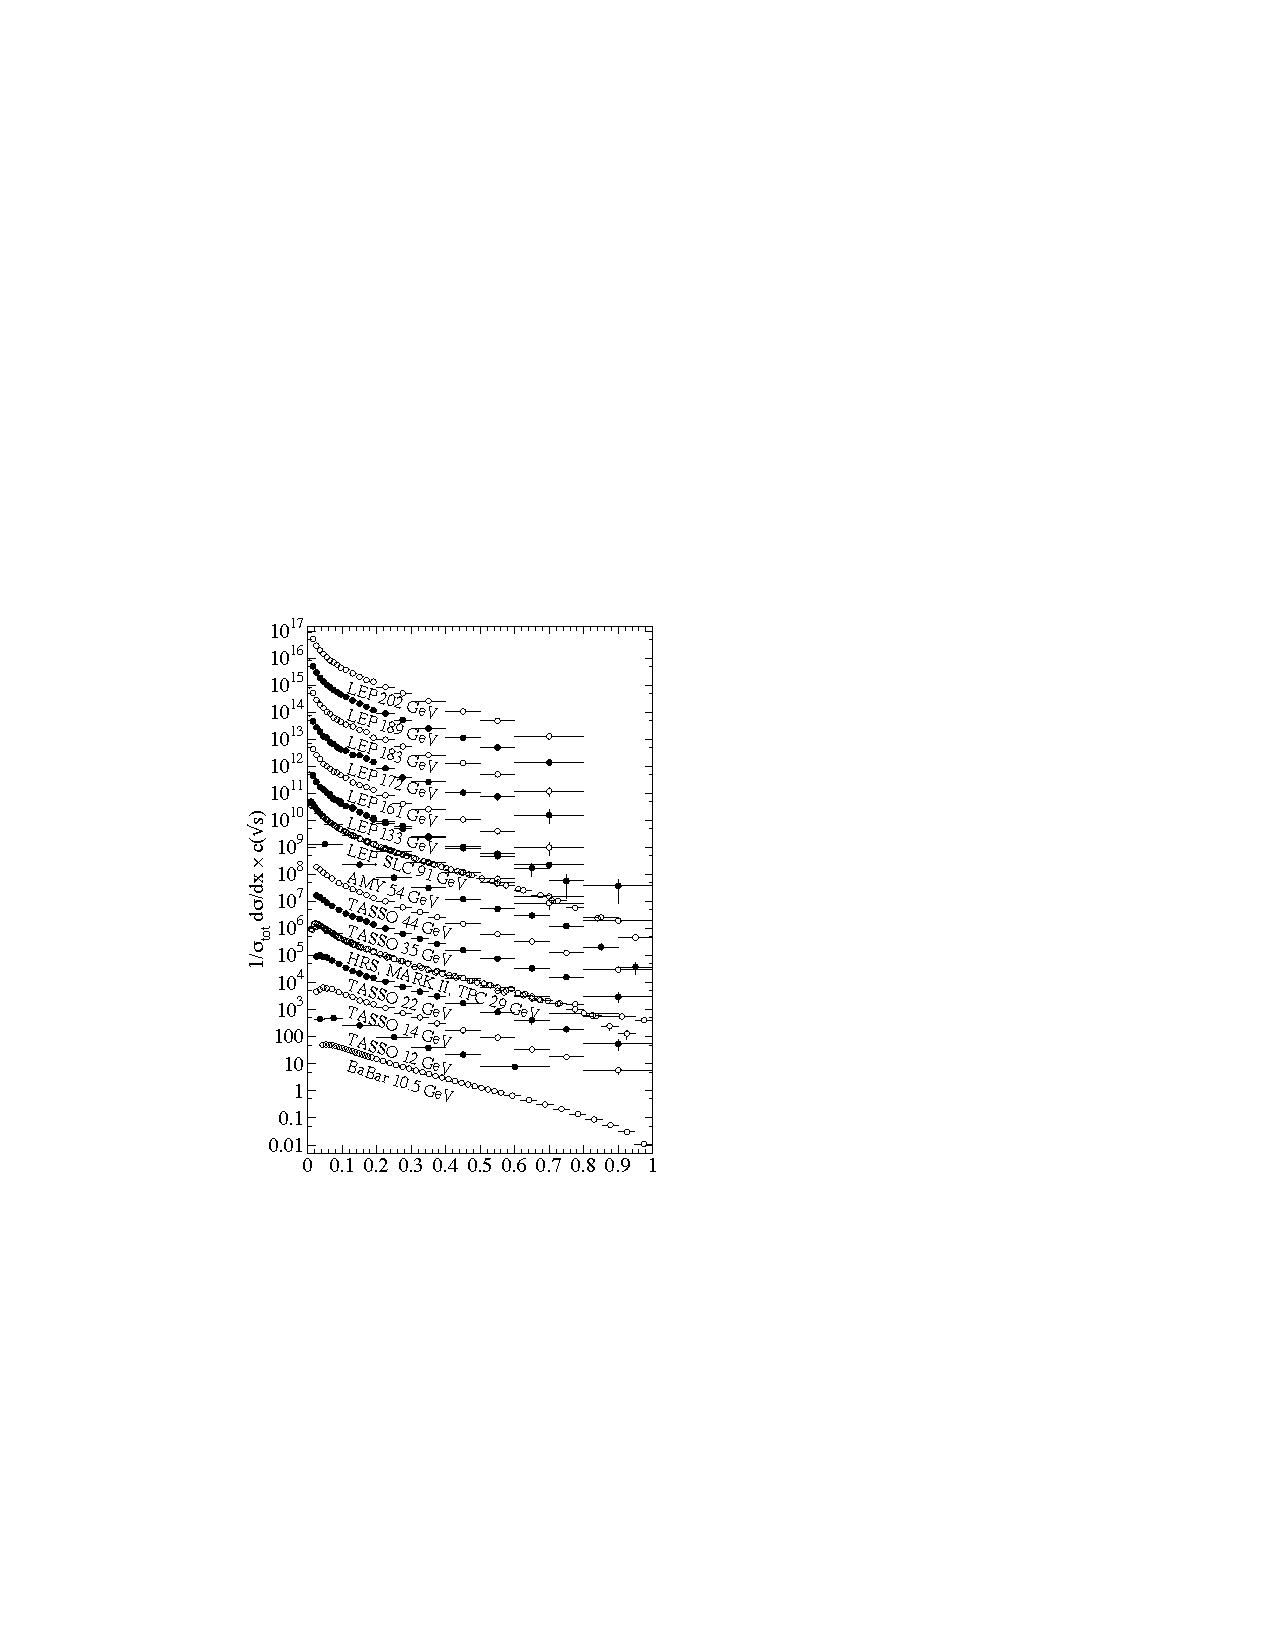
\includegraphics[width=0.8\textwidth]{Introduction/pdg_ff.pdf}
    \caption{The $e^+e^-$ fragmentation function for all charged particles for different CM energies  $ \sqrt{s} $ versus $x$. For the purpose of plotting, the distributions were scaled by  $c(\sqrt{s}) = 10^i$, where $i$ ranges from i=0 ($\sqrt{s}=12$ GeV) to i=13 ($\sqrt{s} = 202 $ GeV) \cite{deFlorian2018}} 
    \label{fig:pdg_ff}
  \end{figure}
  
  \begin{figure}[htpb]
    \centering
    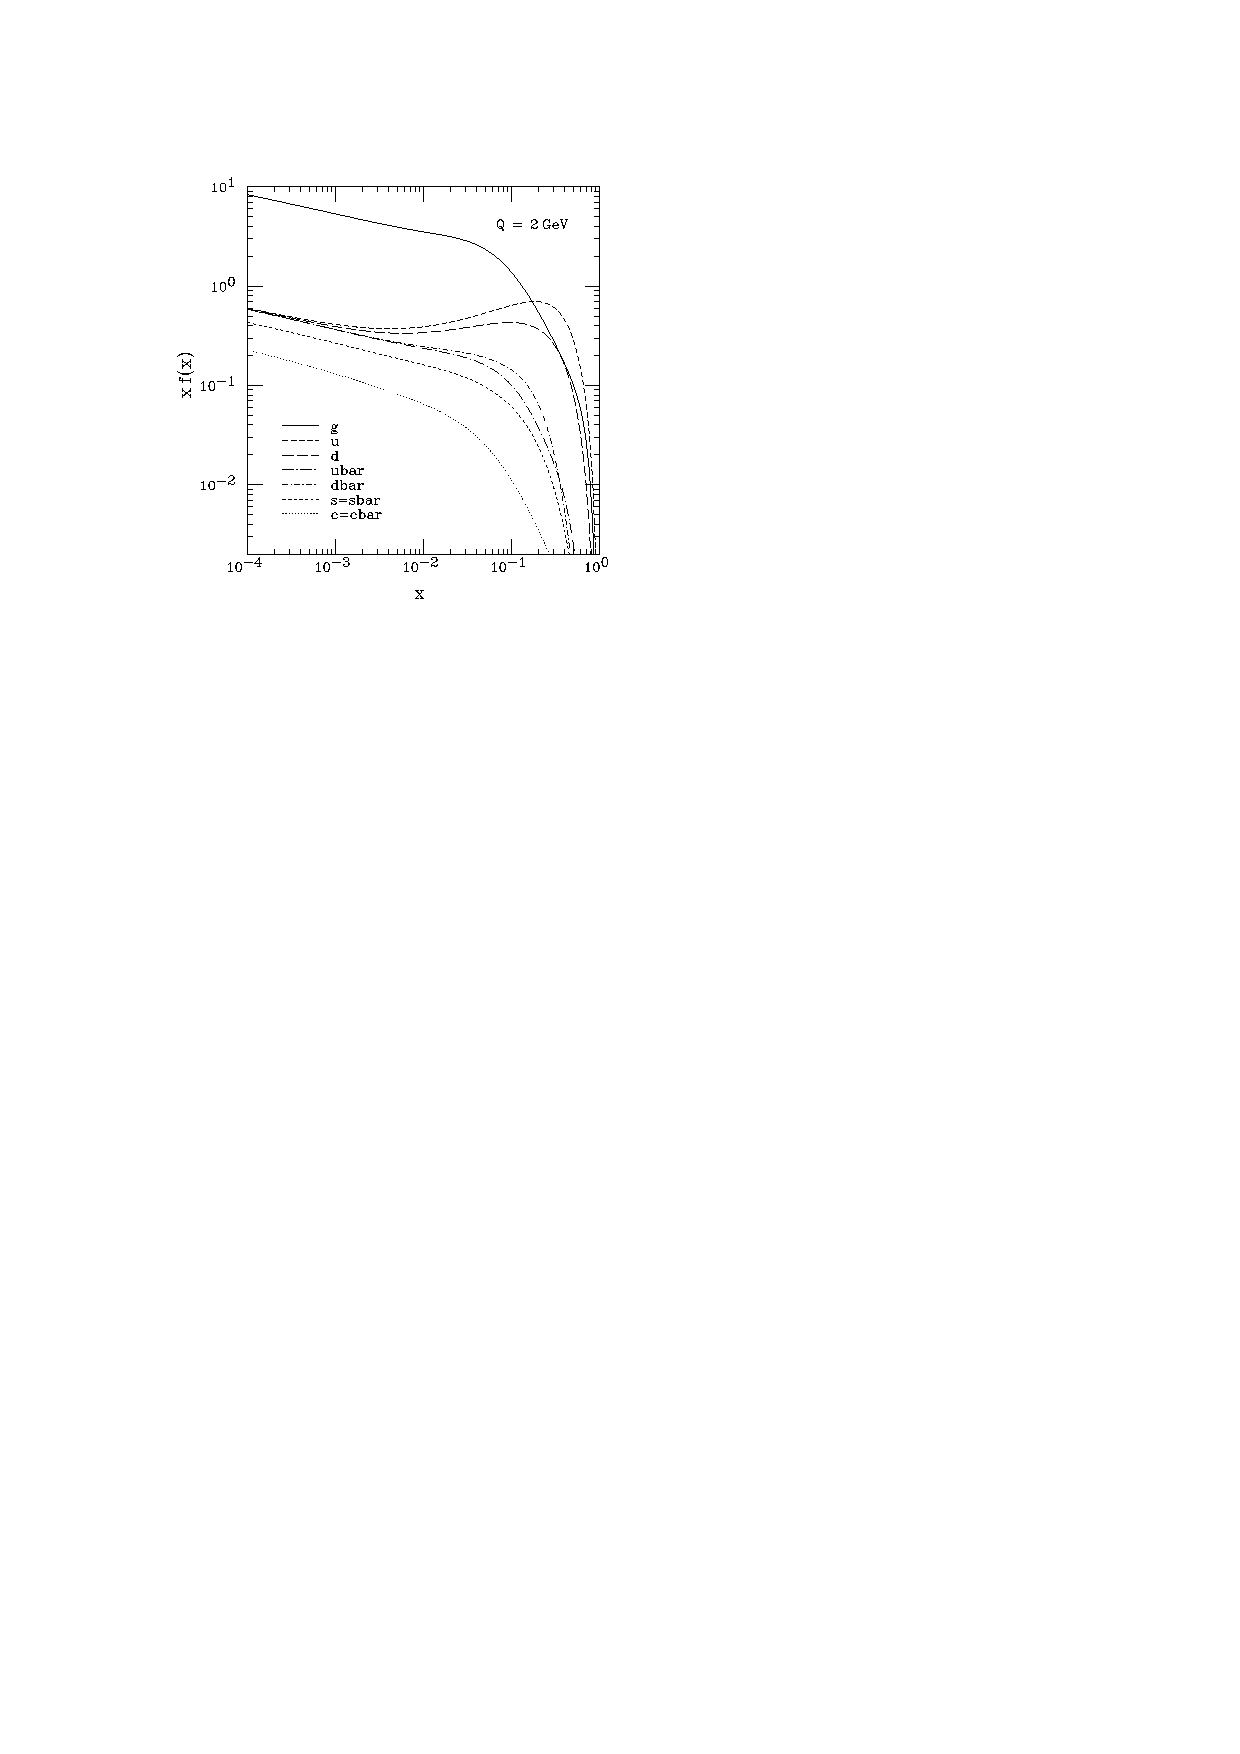
\includegraphics[width=0.8\textwidth]{Introduction/pdfs.pdf}
    \caption{Sampling of PDFs from CTEQ \cite{Pumplin2002}}
    \label{fig:dis_pdfs}
  \end{figure}

In a similar story of progression, p+p collisions are important baseline data for collisions of heavy nuclei, discussed in Sec.~\ref{sec:raa}. It turns out, expectations for hadronic observables must be modified in nuclear collisions. Furthermore, p+Pb collisions are important for disentangling cold and hot nuclear matter effects. Such departures provide a window into physics beyond the vacuum behavior of QCD accessed via elementary particles collisions. 


% \section{Cold Nuclear Matter Effects}\label{sec:coldnm}
% shadowing, kT effect, others\ldots.


\section{Two Particle Correlations}
Another way to study energy loss effects on partons propagating through a medium in heavy ion collisions is by measuring two particle correlations. One of simplest forms of two particle correlations is the di-hadron correlation. Contemporary jet measurements invoke jet reconstruction algorithms to determine the full energy of the jet event-by-event. These methods are difficult to apply in heavy-ion collisions due to the overwhelming background from soft collisions, and may be less sensitive to medium modification depending on the observable being measured. Instead, a very useful approach has been to measure correlations between particles.

\begin{equation}
    Y(\deltaphi)\equiv \frac{1}{n^\mathrm{triggers}}\frac{\mathrm{d}N}{\mathrm{d}\deltaphi}
    \label{eq:yield}
  \end{equation}

$N$ is the number number of correlated particles, $n^\mathrm{triggers}$ is the measured number of triggers, and  $\dphi$ is the difference in azimuthal angle between the trigger and associated particle. Fig.~\ref{fig:dihadron_cartoon} shows a simplified example of a di-hadron (hadron-hadron, or h-h) correlation in p+p collisions. The two-peak structure is characteristic of such measurements, and indicates that the event sample is dominated by di-jet events. The particles within the same jet make up the narrow peak centered around \deltaphi~= 0 and the recoil jet appears as the peak around $\deltaphi = \pi$. The away side peak is broadened since kinematically the away side jet can swing along the $\eta$ direction and $k_\mathrm{T}$, the initial pair momentum of the colliding partons, can create an imbalance in the jets’ energy and cause them to be acoplanar. $\eta$, also referred to as psuedorapidity, is defined as $\eta = \ln(\tan(\theta/2))$, where $\theta$ is the polar angle with respect to beam direction. A 2D plot ($\deltaphi,\Delta\eta$) of this correlation in pPb and pp collisions is shown in Fig.~\ref{fig:near_side_ridge}, Sec.~\ref{sec:flow}. The peaks sit atop a pedestal which is due to initial and final state interactions amongst the beam remnants and the hard-scattered partons. This must be subtracted, and will be discussed in greater detail in Sec.~\ref{sec:ue_subtraction} for pp and pPb collisions. For AA collisions, this subtraction is even more complicated, where flow is no longer a signal, but a background phenomenon that must be subtracted. 

  \begin{figure}[htpb]
    \centering
    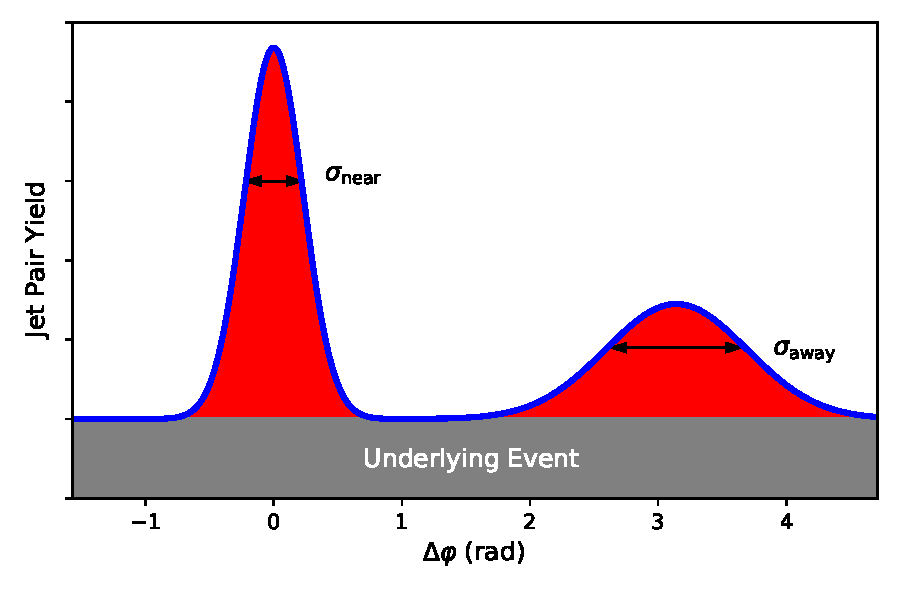
\includegraphics[width=0.8\textwidth]{Introduction/dihadron_cartoon.pdf}
    \caption{Cartoon illustrating a measurement of two-particle correlations from jets}
    \label{fig:dihadron_cartoon}
  \end{figure}

  The STAR experiment performed a hadron-hadron correlation measurement with triggers of $p_{\mathrm{T},t}>$ 4 GeV/$c$ and associated partners of 2 GeV$/c<p_{\mathrm{T},a}<p_{\mathrm{T},t}$. The result, shown in Fig.~\ref{fig:dihadron_correlation} demonstrates that for central Au + Au collisions the near-side jet looks very similar to p+p but the away-side jet completely disappears. This is consistent with a picture in which the near-side jet is usually produced near the surface and the away-side jet is completely absorbed by the medium.

  \begin{figure}[htpb]
    \centering
    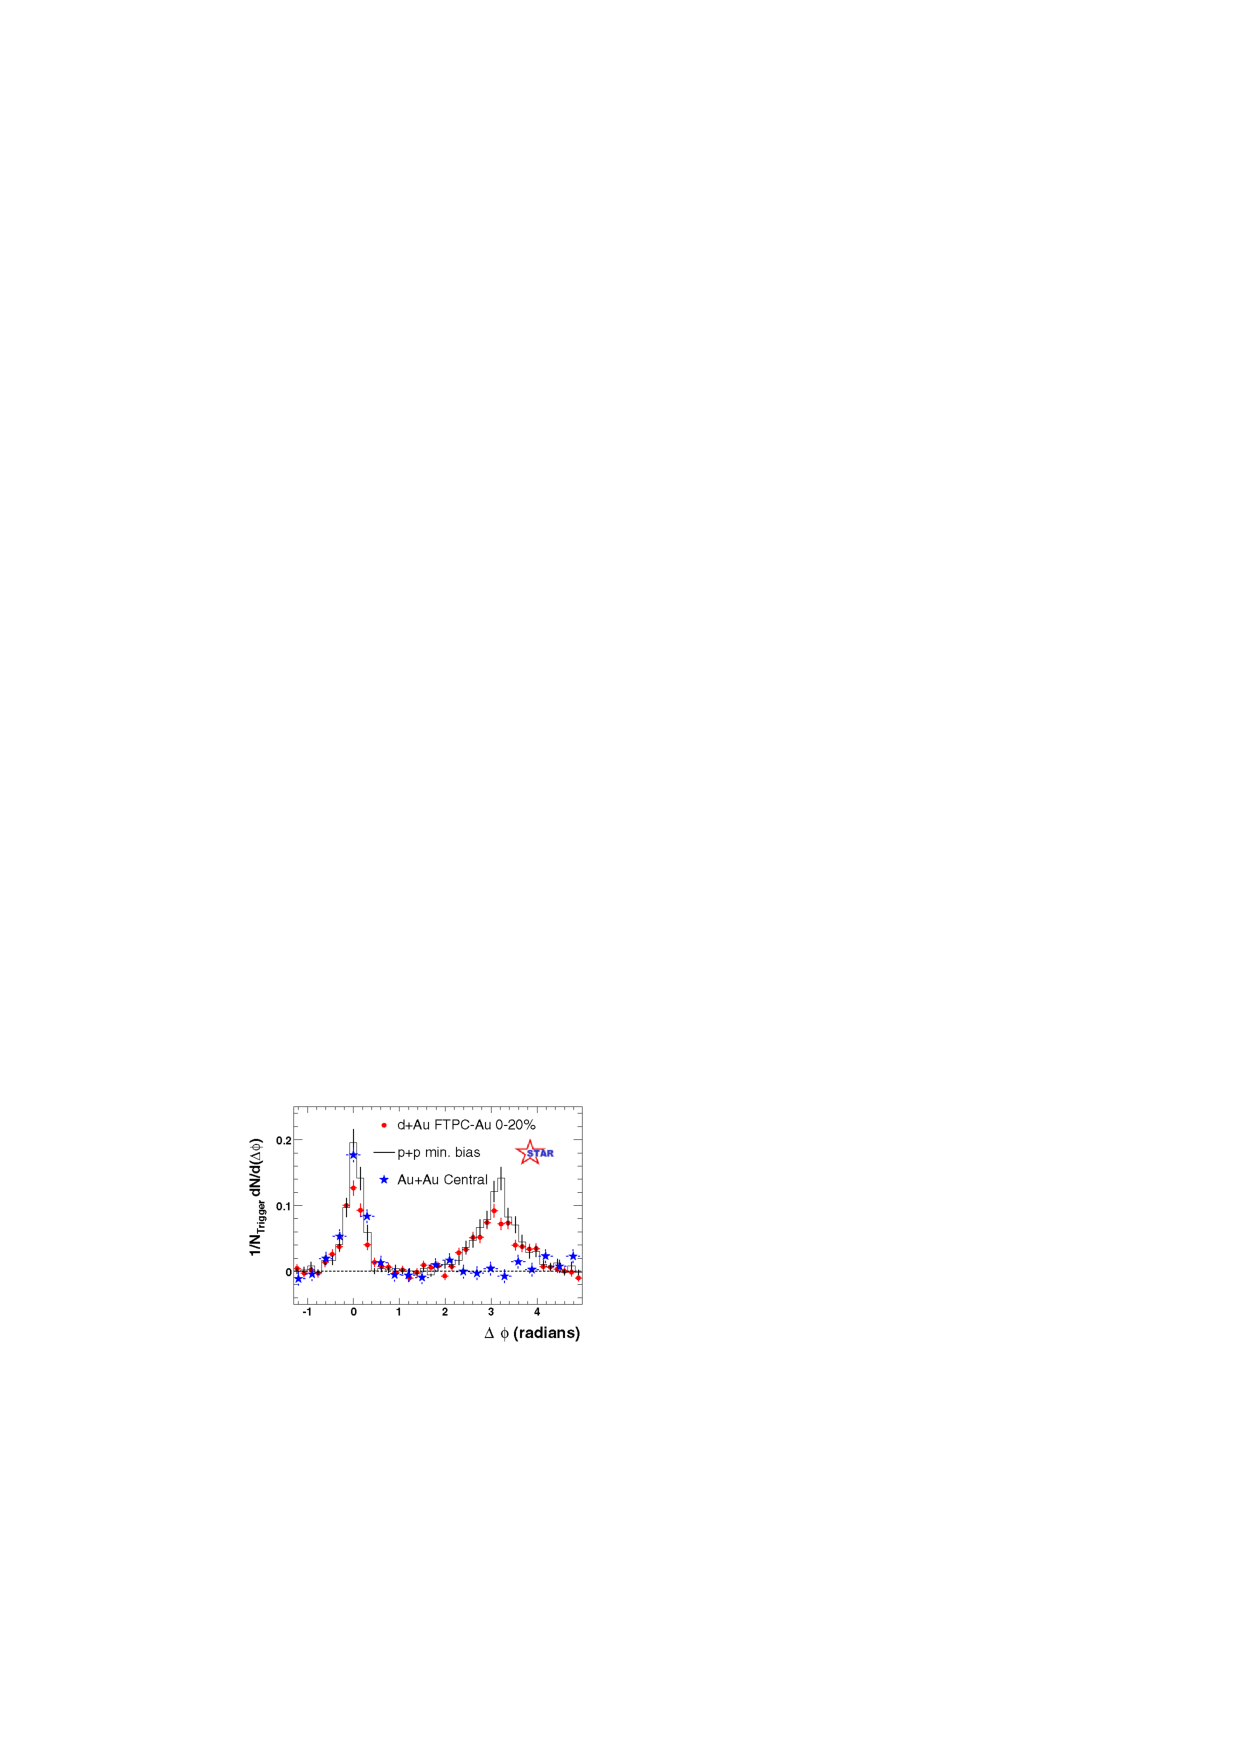
\includegraphics[width=0.8\textwidth]{Introduction/star_dihadron.pdf}
    \caption{Hadron-hadron correlations measured in p+p, d+Au and Au+Au collisions at STAR. The near side jet peaks around $\deltaphi$=0 in all three systems but the away-side which peaks around $\deltaphi=\pi$ in p+p and d+Au, is suppressed in Au+Au \cite{Adams2005}.}
    \label{fig:dihadron_correlation}
  \end{figure}

Although hadron-hadron correlations have revealed a great deal about energy loss in the medium, they are limited by the fact that the initial parton momentum is unknown and cannot be used to directly measure the fragmentation function.

\section{Prompt Photons}
Prompt photons can be defined simply as the photons produced immediately in the collision, before final state hadrons are produced. At the lowest order in pQCD, prompt photons are produced via two processes: (i) quark-gluon Compton scattering, $qg \to q\gamma$, (ii) quark-antiquark annihilation, $q\overline{q} \to g\gamma$, and, with a much smaller contribution,  $q\overline{q}\to$ $\gamma\gamma$. In p+p collisions, the Compton-type process dominates the cross section by roughly an order of magnitude over annihilation as a result of the scarcity of antiquarks. Additionally, prompt photons can be produced in higher-order processes, such as fragmentation or bremsstrahlung \cite{Aurenche1993}. The collinear part of such processes has been shown to contribute effectively also at lowest order. The basic Feynman diagrams for these processes (excluding $q\overline{q}\to$ $\gamma\gamma$) are shown in Fig.~\ref{fig:prompt_feynman}.

\begin{figure}[htpb]
  \centering
  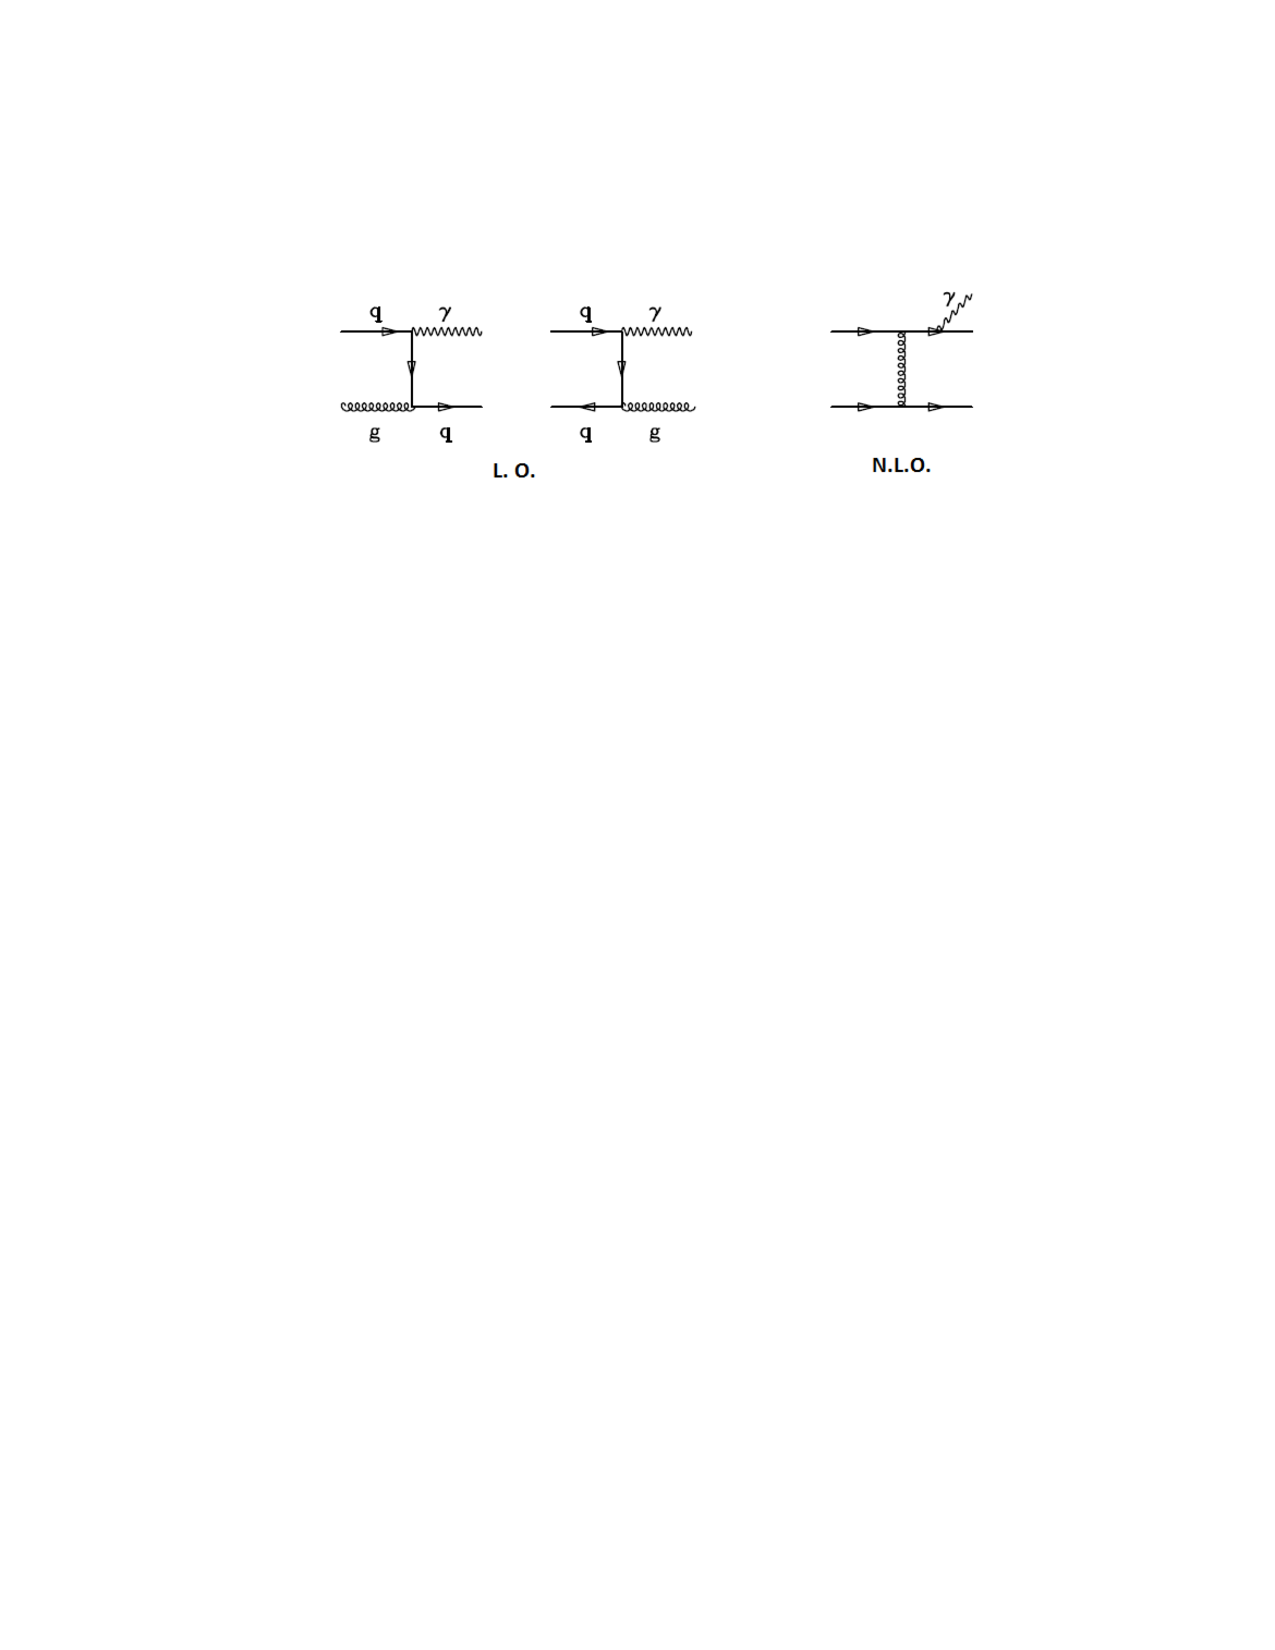
\includegraphics[width=0.8\textwidth]{Introduction/prompt_photons.pdf}
  \caption{On the left are the leading order Feynman diagrams for direct photon production. The diagram on the right is next-to-leading order. Photons resulting from this diagram are referred to as fragmentation photons}
  \label{fig:prompt_feynman}
\end{figure}

%ALICE-Prompt: Photons not from hadronic decays
%PHENIX-Prompt: RIGHT FROM THE COLLISION (excludes fragmentation)
%Direct is the same in both cases.
%%%%%LEADING ORDER FEYNMAN DIAGRAMS FROM QUAL%%%%%%%%%

Photons produced during fragmentation, are aptly named fragmentation photons. As a result, fragmentation photons are often surrounded by a larger amount of energy and hadronic activity than other prompt photons produced from the initial hard scattering.

Prompt photons, and by extension fragmentation photons, are both included in the definition of direct photons. While the definition of direct photons is not always consistent in the literature, and varies slightly between experiments, we define direct here to mean any photon not produced from hadronic decays. Those photons originating from the decay of a hadronic bound state are defined as decay photons. The two largest sources of decay photons are the two-photon decay channels of the $\pizero$ and $\eta$ meson. At higher \pt, decay photons make up the majority of photons produced in the collision.

Together, direct and decay photons make up all the photons observed in a collision, called inclusive photons.

\begin{equation}
  \gamma_\mathrm{inclusive} = \gamma_\mathrm{direct} + \gamma_\mathrm{decay}
\end{equation}

\section{Photons in Heavy Ion Collisions}
Direct photons have three very important properties that make them valuable tools in heavy-ion physics. First, There are relatively few leading order diagrams which contribute to direct photon production. Second, The photon-quark coupling is point-like, and not effected by long-range QCD behavior such as fragmentation in the final state. Third, though a property shared with other high-\pt~photons, they do not interact with the QGP. Prompt photons are extremely valuable tools in heavy-ion physics. One property that makes them so useful is that they are not expected to interact with the QGP.

Photons do not carry color charge, and should therefore be unmodified by strong interactions in a medium. While the plasma is made up of quarks that carry (fractional) charge, For example, the mean free path of a 1 GeV photon in a QGP at $T=$200 MeV was calculated to be  $\lambda=480$ fm, much larger than the estimate size of plasma at  $r \approx 10$ fm~\cite{David2020}.

Thus, in the leading order picture, after prompt photons are produced early in the collision they should propagate through the medium completely unmodified, with no high \pt~suppression. This has been verified, by measuring the $R_\mathrm{AA}$ of photons, shown in Fig.~\ref{fig:photon_raa}.

\begin{figure}[htpb]
  \centering
  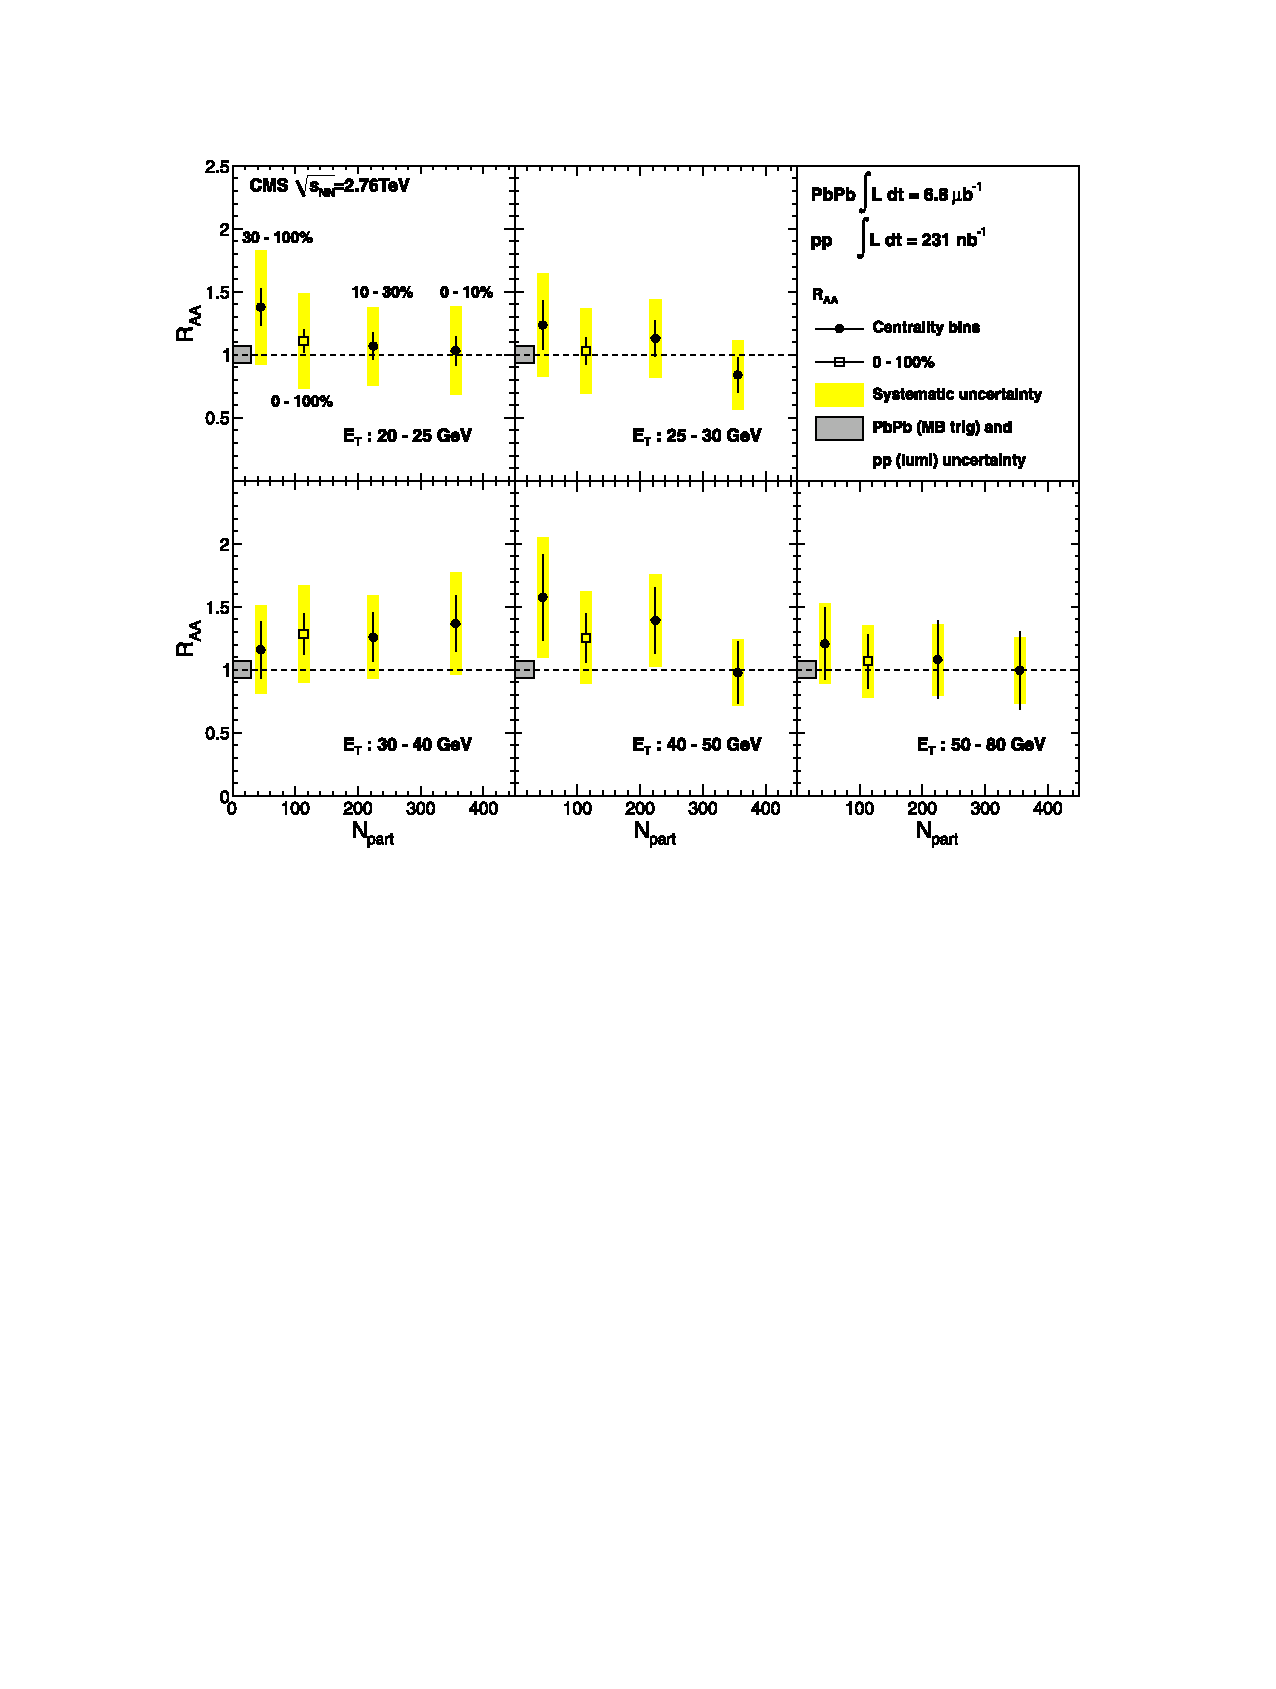
\includegraphics[width=0.8\textwidth]{Introduction/photon_raa}
  \caption{The measured nuclear modification factor $R_\mathrm{AA}$ as a function of PbPb centrality (given by the number of participating nucleons,$N_\mathrm{part}$) for five different photon transverse energy ($E_\mathrm{T}$) intervals.}
  \label{fig:photon_raa}
\end{figure}

A measured $R_\mathrm{AA}$ consistent with 1.0 strongly supports the position that photons are unmodified in the quark gluon plasma.

% For γ − h correlations, on the other hand, the conditional yield should be much more closely related to the fragmentation function. In the leading order picture, the direct photon exactly balances the away-side jet and therefore, the measurable quantity, pT,a/pT,t, is nothing but the fragmentation variable pT,a/pT,jet. This explains why γ − h correlations are a powerful measurement. They provide a source of recoil partons of fixed momentum. Their conditional yields in p + p collisions only probe the jet fragmentation. By contrast, hadron correlations are controlled by the jet cross section which also depend on the PDF’s and the parton scattering cross sections.

\subsection{$\gamma$-Jet Correlations}
\label{sec:intro_gj}
Another important property of leading order prompt photons is that the photon-quark coupling is point-like and therefore not complicated by long-range QCD behavior such as jet fragmentation in the final state, in distinction to hadronic observables. Thus, in the leading order picture, the direct photon exactly balances the away-side parton and resulting jet. Here the photon acts as a reference to the parton from the initial scattering, before any modification in heavy-ion collisons. This means that comparisons between the photon and parton, or jet, as well as large deviations from \deltaphi~$\approx\pi$ can be used to directly study medium-induced effects on the recoiling parton. $\gamma$-jet correlations in CMS are shown in Fig.~\ref{fig:cms_gj_correlations}~\cite{Sirunyan2018}.


\begin{figure}[htpb]
  \centering
  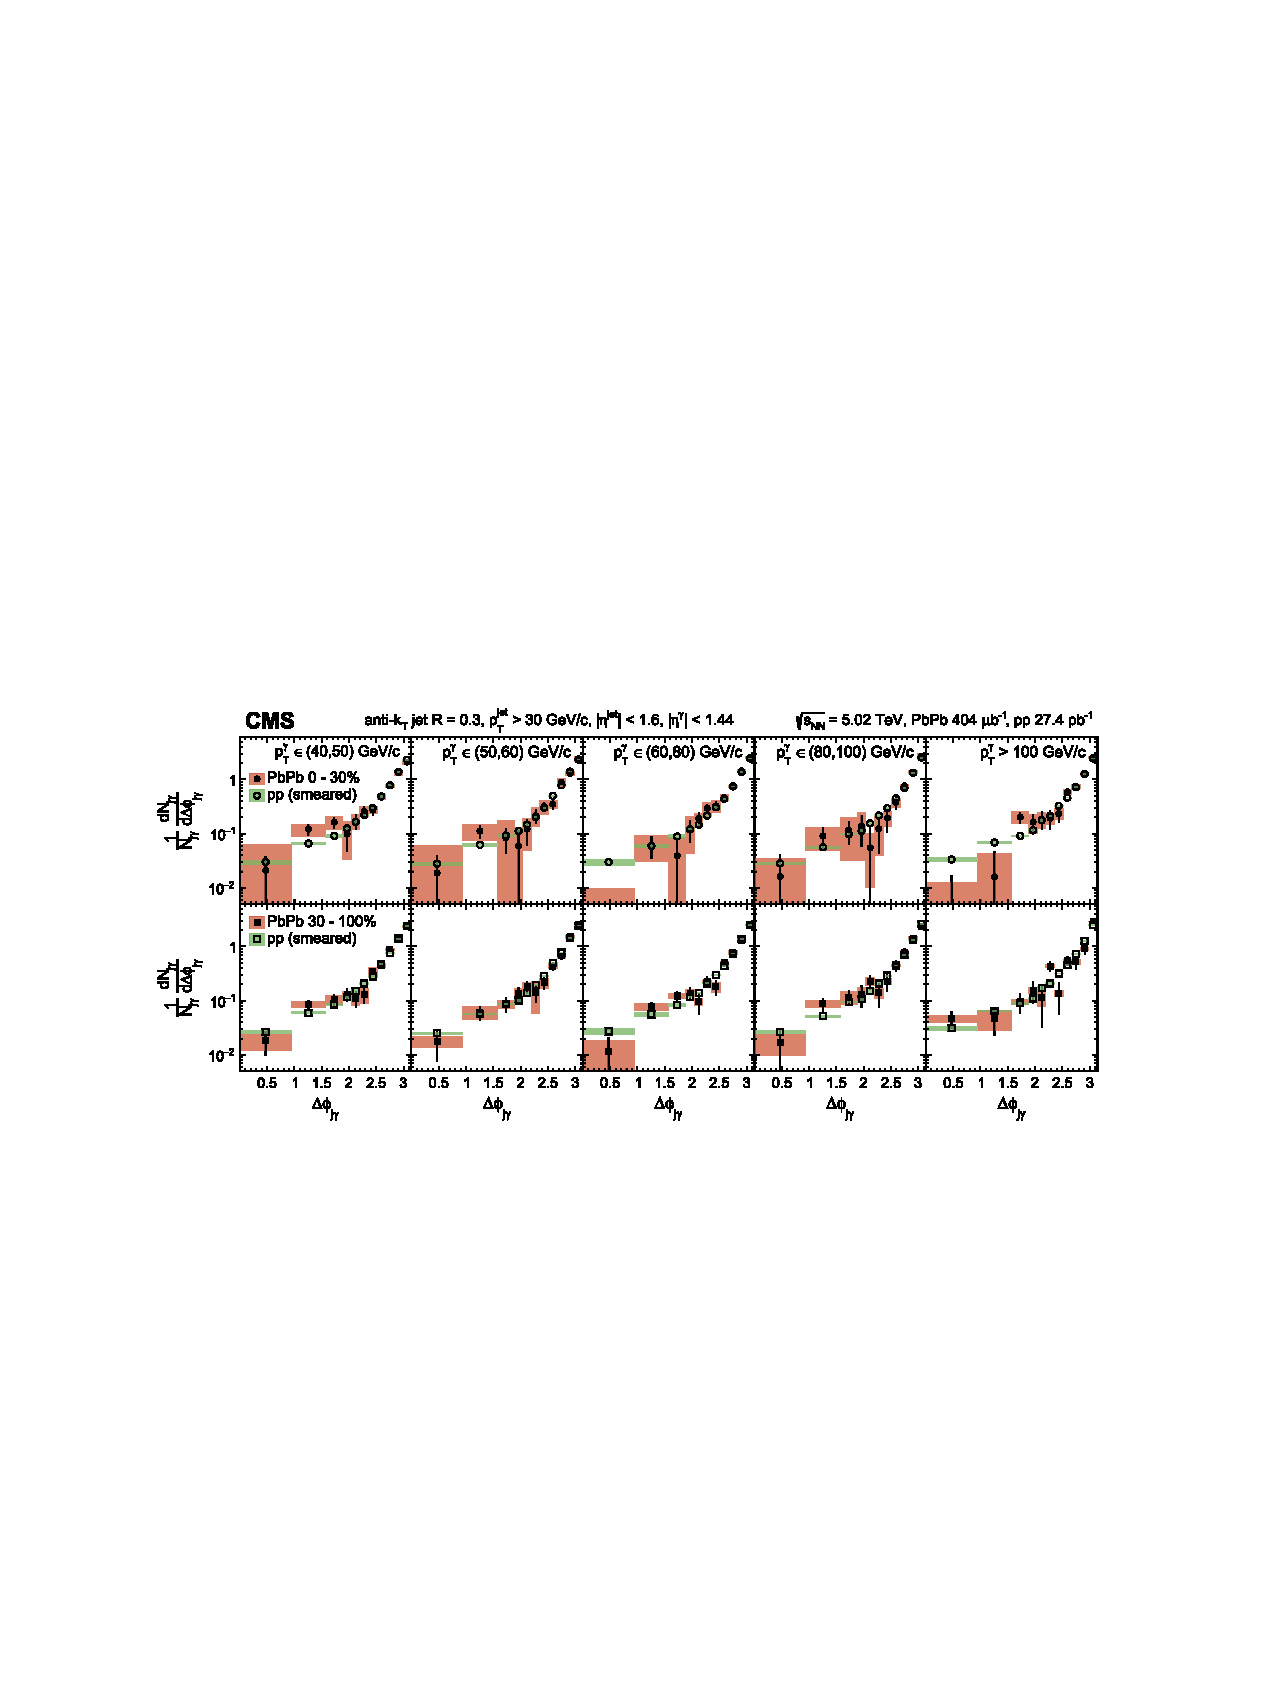
\includegraphics[width=0.99\textwidth]{Introduction/cms_gj_correlations.pdf}
  \caption{The azimuthal correlation of photons and jets in five $\pt^\gamma$ intervals for 0–30\% centrality (top, full circles) and 30–100\% centrality (bottom, full squares) PbPb collisions. The smeared pp data (open symbols) are included for comparison. The vertical lines (bands) through the points represent statistical (systematic) uncertainties \cite{Sirunyan2018}.}
  \label{fig:cms_gj_correlations}
\end{figure}


In conjunction with $\gamma$-jet correlations, the $\gamma$-jet asymmetry, $x_{j,\gamma}\equiv \pt^\mathrm{jet}/\pt^\gamma$ can be measured to quantify in-medium parton energy loss. Derived from Fig.~\ref{fig:cms_gj_correlations}, the jet asymmetry for jets with $\deltaphi > 7\pi/8$ relative to the photon were taken. The asymmetry as a function of photon \pt, as well as the ratio of yields for large $\deltaphi$, $R_\mathrm{AA}$, is shown in Fig.~\ref{fig:cms_gj_quenching.pdf}~\cite{Sirunyan2018}.

\begin{figure}[htpb]
  \centering
  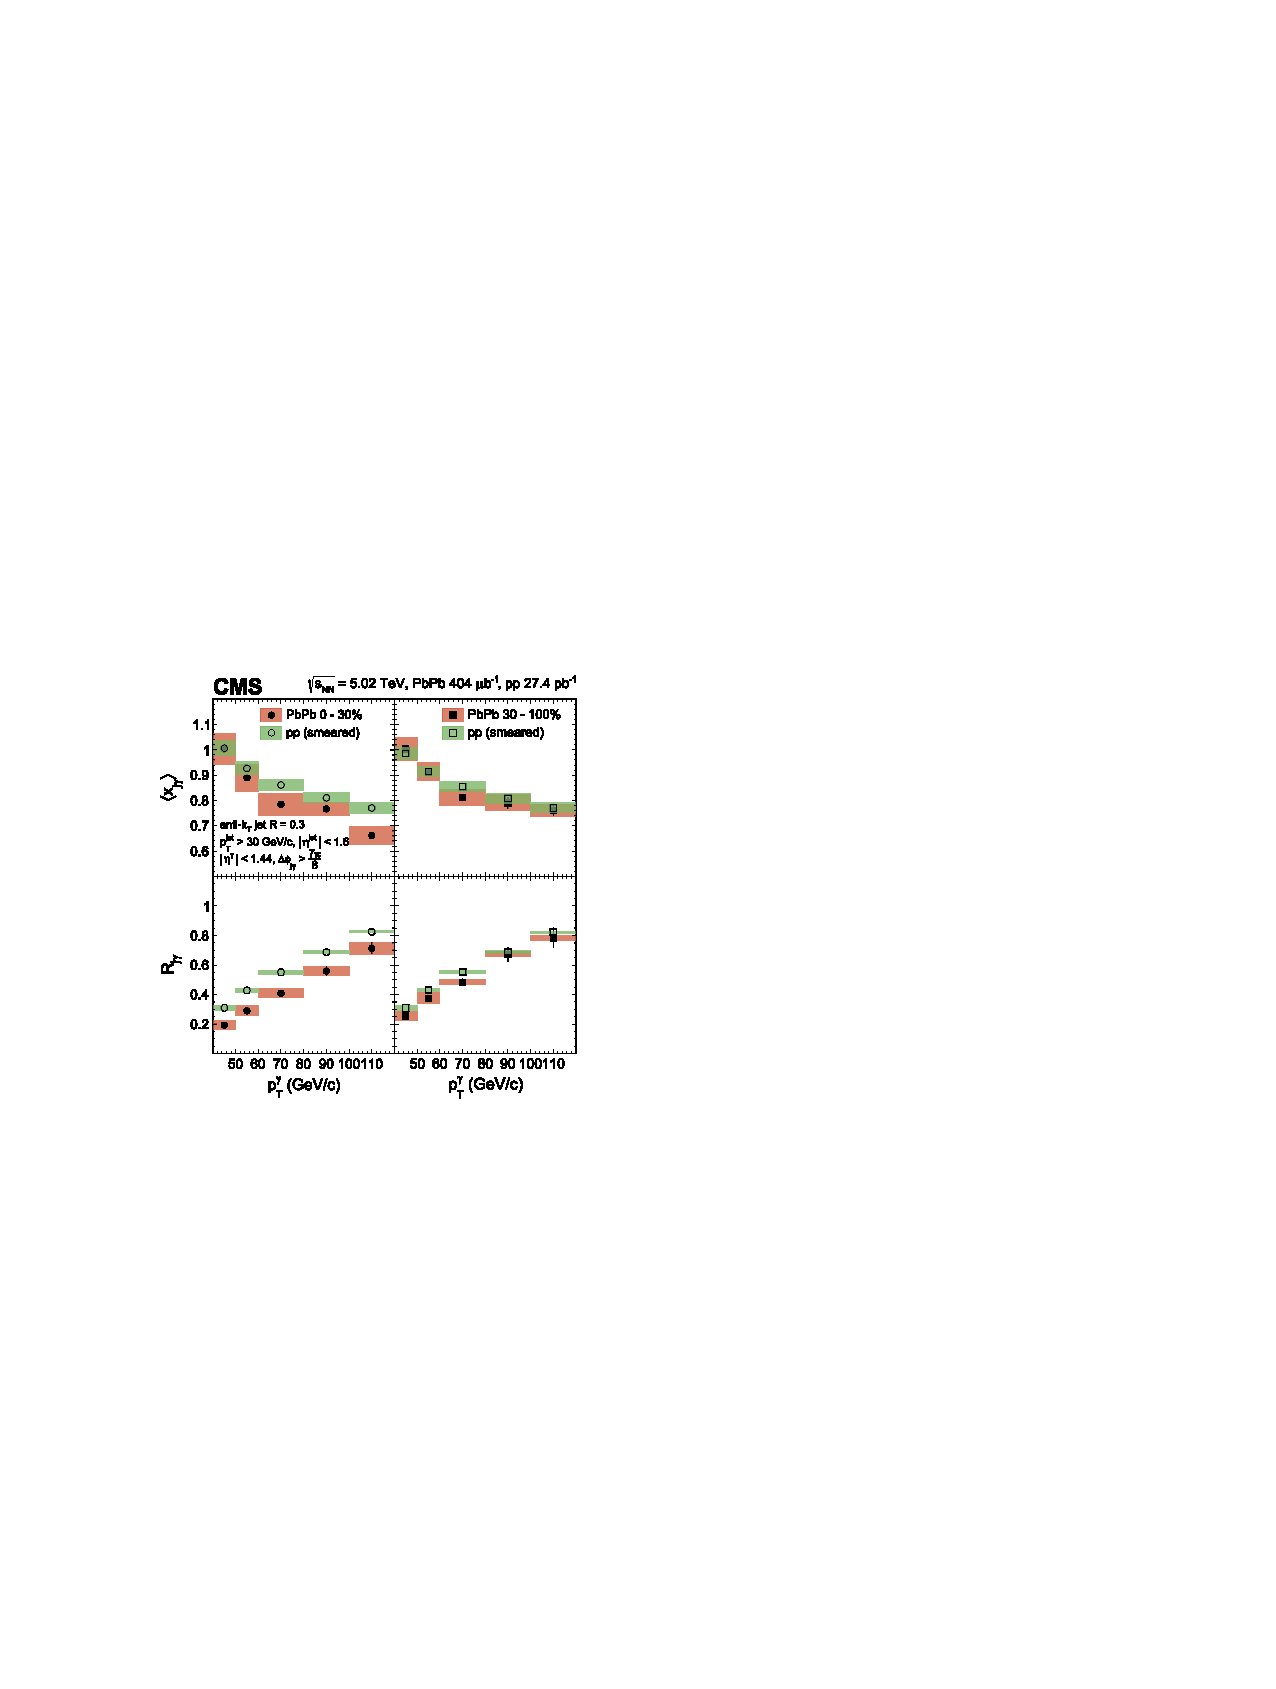
\includegraphics[width=0.8\textwidth]{Introduction/cms_gj_quenching.pdf}
  \caption{The $\langle x_{j,\gamma} \rangle$ values (top) and $R_\mathrm{j\gamma}$, the number of associated jets per pho-ton (bottom), in 0–30\% centrality (left, full circles) and 30–100\% centrality (right, full squares) PbPb collisions. The smeared pp data (open symbols) are added for comparison. The vertical lines (bands) through the points represent statistical (systematic) uncertainties.}
  \label{fig:cms_gj_quenching.pdf}
\end{figure}

This procedure from CMS also provides a good example of how these correlations are often used to extract other measurements: The angular correlations are measured, from which a region in large $\deltaphi$ is taken (corresponding to the photon and parton being back-to-back). The yields in this region are then reported as a function of fractional momentum, $x_{j,\gamma}$ in order to measure medium effects.

\subsection{$\gamma$-hadron Correlations}
\label{sec:intro_gh}
The leading order picture of prompt photons indicates that the photon and recoiling parton have equal and opposite transverse momenta. Therefore, the measurable quantity, $\zt = p_{\mathrm{T},a}/p_{\mathrm{T},t}$ with the prompt photon as the trigger,  is nothing but the fragmentation variable, $p_{\mathrm{T},hadron}/p_{\mathrm{T},parton}$. This explains why prompt $\gamma$-h correlations are such a powerful measurement. They provide a source of recoil partons of fixed momentum and their conditional yields as a function of \zt in p+p collisions probe the parton fragmentation. By contrast, dihadron correlations are controlled by the jet cross section which also depend on the PDF’s and the parton scattering cross sections. 

When the hadrons roughly opposite the trigger photon are reconstructed as a jet, they are clearly connected to the recoiling parton from the initial scattering in the leading order picture. The hadrons within those jets can then be used to probe the jet fragmentation function. $\gamma$-hadron correlations in which a jet is not reconstructed, however, have a distinct advantage over $\gamma$-jet correlations: hadrons are more sensitive to in-medium modification. Fig.~\ref{fig:raa_particles} shows a minimum in $R_\mathrm{AA}$ for charged hadrons at approximately 6GeV, and a plateau begins after 20 GeV$/c$. It is extremely difficult to measure jets below around 20 GeV/$c$ in heavy ion collisions due to the large background \cite{STARCollaboration2017}. Selecting jets at higher \pt~(or jets with kinematics similar to that in ''vacuum'', or pp collisions), to avoid this background biases the jet population towards jets that will lose the least energy in vacuum, as discussed in Sec.~\ref{sec:raa}. Additionally, triggering on a high \pt~hadron as a proxy for a jet can bias the measurement towards jets towards the surface of the medium \cite{Zhang2007}. Similar to $R_\mathrm{AA}$, the ratio of the conditional yields for $\gamma$-h and $\gamma$-jet correlations in pp and AA collisions can help quantify medium induced modifications to the parton, in this case, the fragmentation function. Fig.~\ref{fig:phenix_gh_corr} shows the direct\footnote{Direct is used in lieu of prompt at RHIC due to the smaller contribution of fragmentation photons at the lower center of mass energies compared to LHC.} photon-hadron correlations measured with the PHENIX detector as a function of $\xi\equiv\ln(1/\zt)$:

\begin{figure}[htpb]
  \centering
  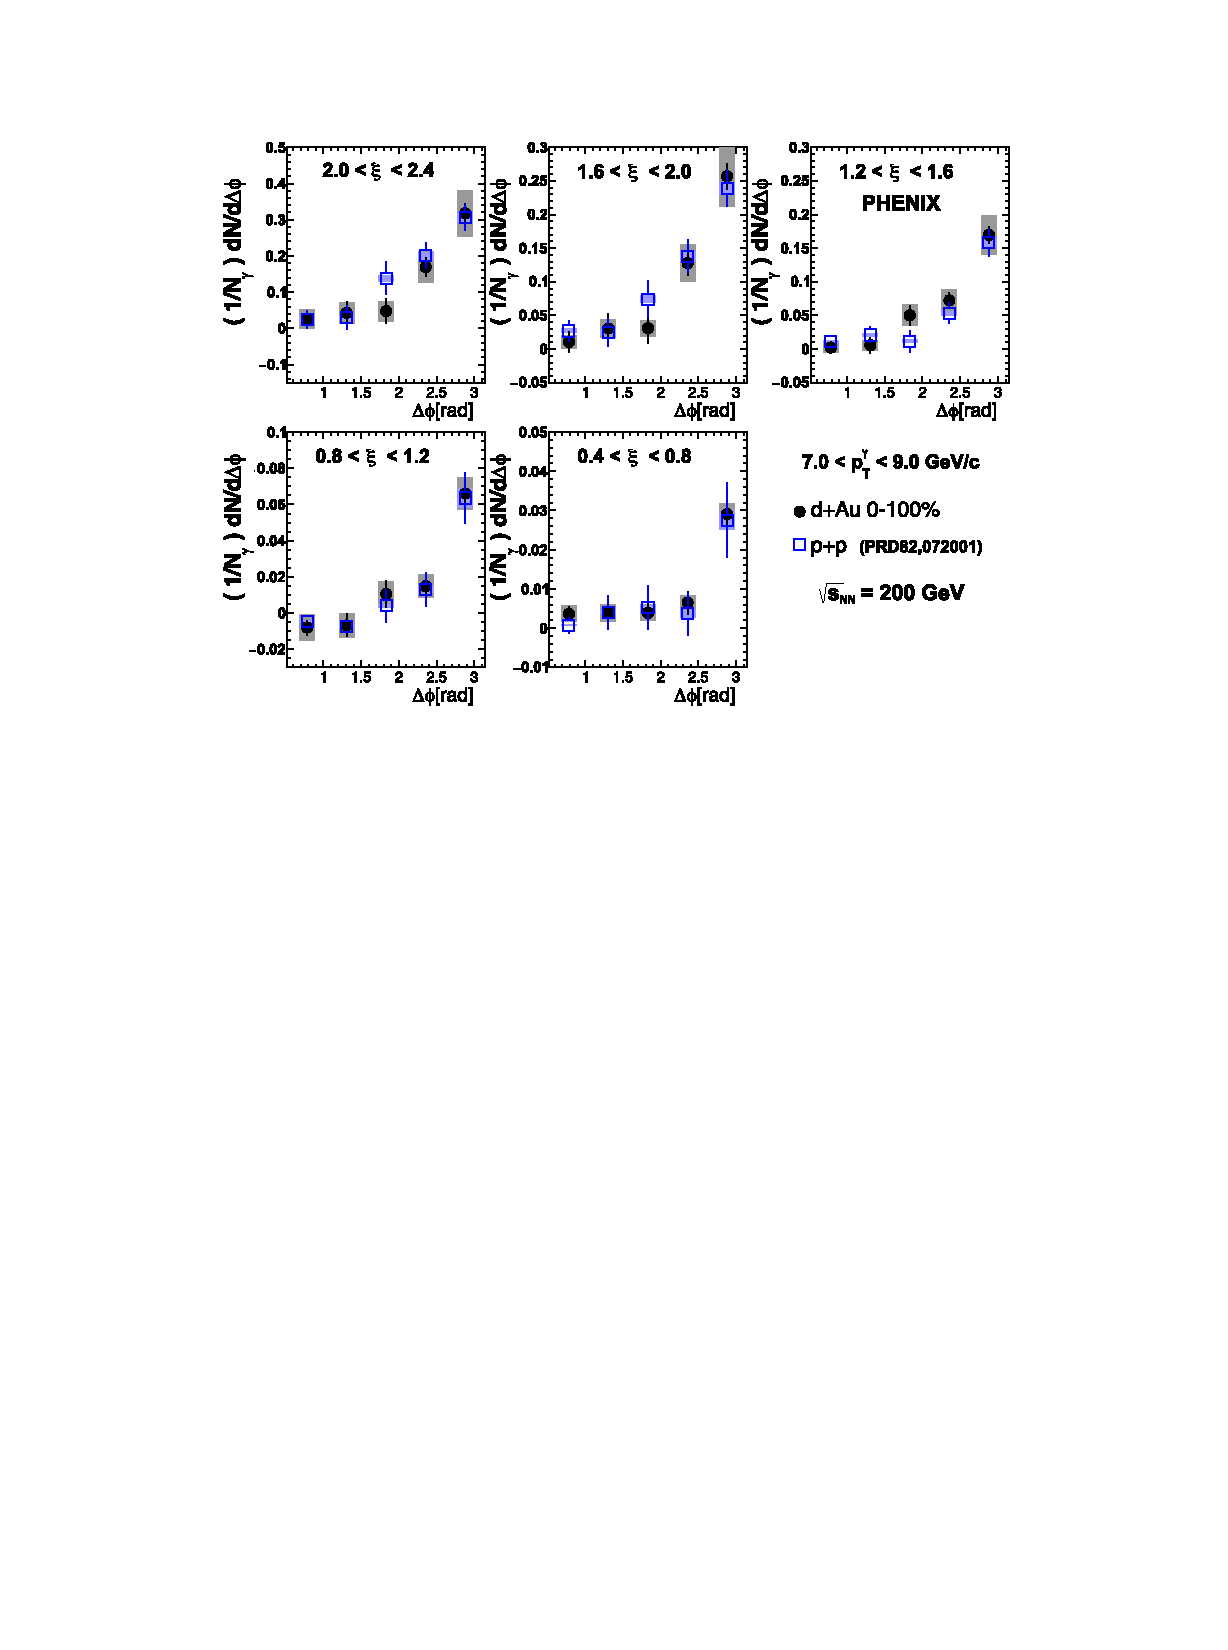
\includegraphics[width=0.8\textwidth]{Introduction/phenix_gh_corr.pdf}
  \caption{Per-trigger yield of hadrons associated with direct photons in Au+Au collisions (closed [black] circles) for direct photon \pT~ 5–9GeV/$c$,compared with p+p baseline (open [blue] squares), in various $\xi$ bins \cite{PHENIXCollaboration2020}.}
  \label{fig:phenix_gh_corr}
\end{figure}

Similar to the $\gamma$-jet measurement in the previous section, the conditional yield at higher \deltaphi~is measured. This conditional yield as a function of $\xi$ is the experimentally measured fragmentation function. The ratio of this yield in pp and AA collisions, $I_\mathrm{AA} \equiv Y_\mathrm{AA}/Y\mathrm{pp}$, is a nuclear modification factor which quantifies the difference between the fragmentation functions in AA and p+p collisions. This is shown in Fig.~\ref{fig:phenix_gh_IAA} \cite{PHENIXCollaboration2020}. 

\begin{figure}[htpb]
  \centering
  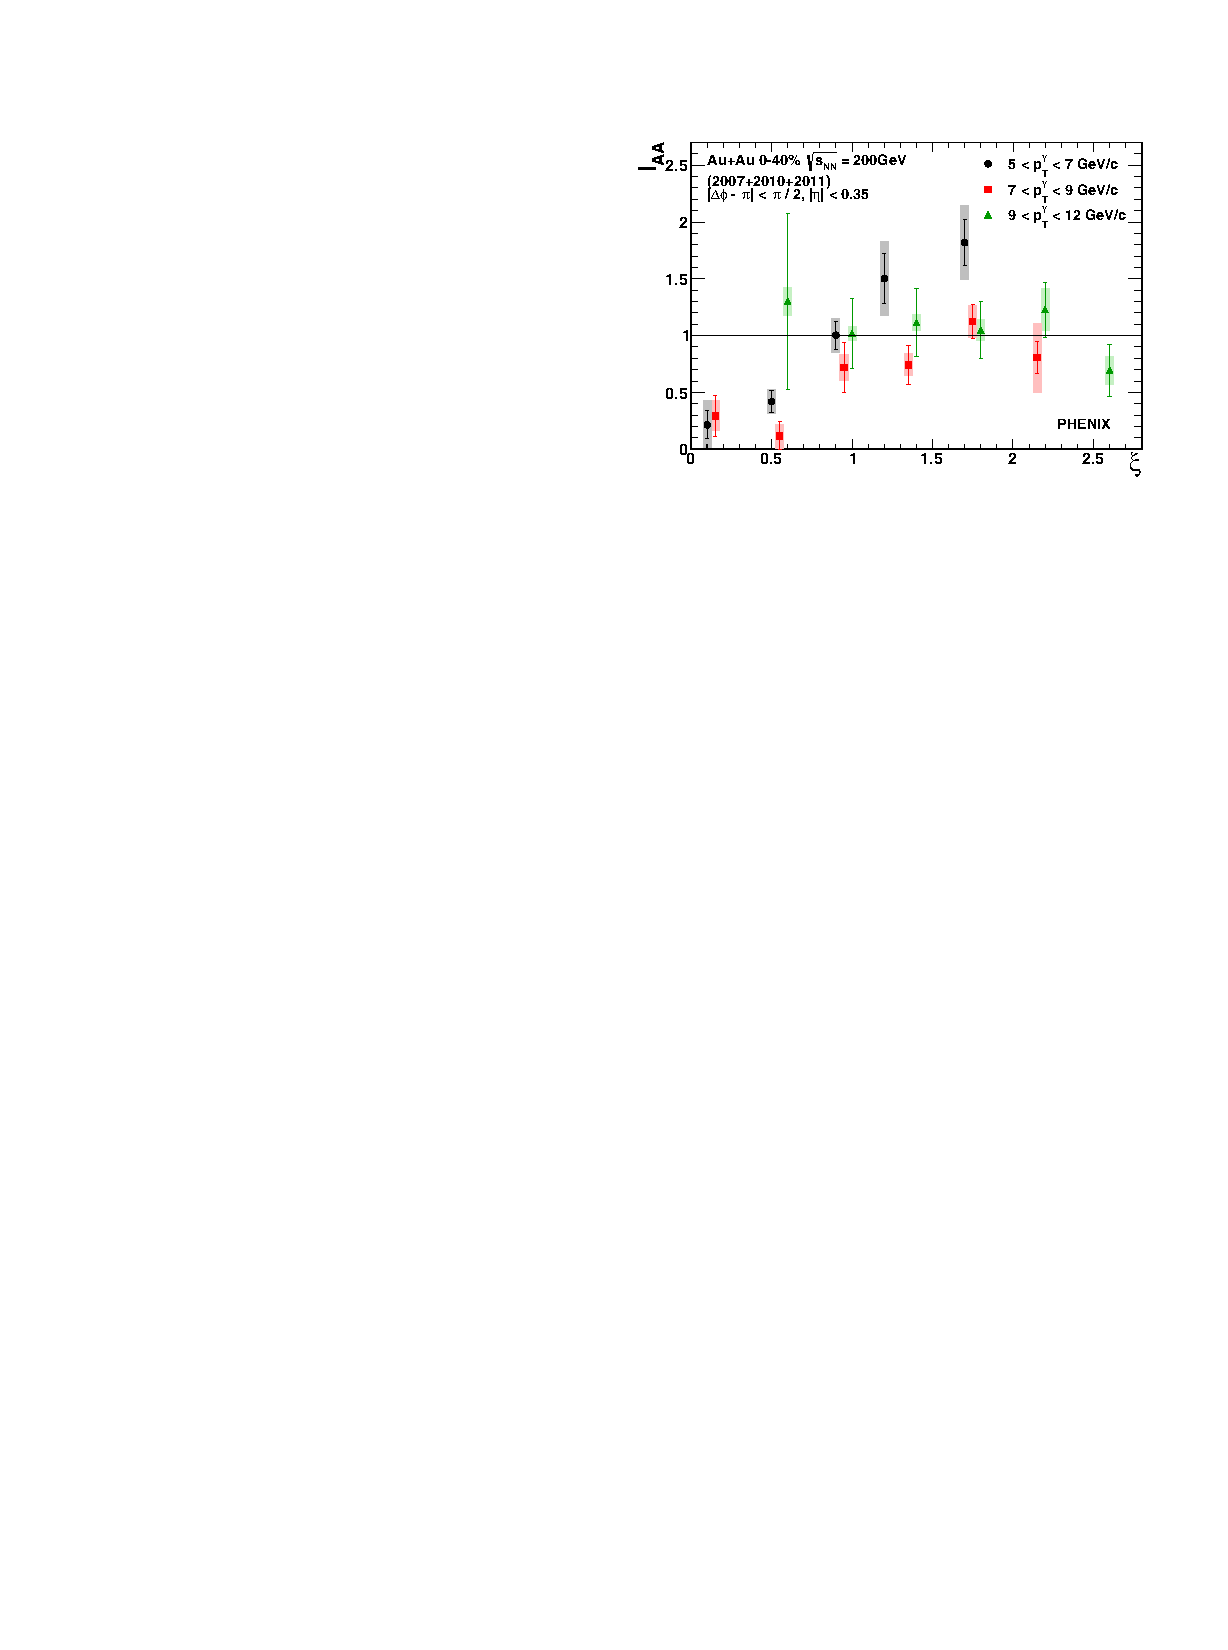
\includegraphics[width=0.8\textwidth]{Introduction/phenix_gh_IAA.pdf}
  \caption{$I_\mathrm{AA}$ for three direct photon $\pt^\gamma$ bins.}
  \label{fig:phenix_gh_IAA}
\end{figure}


$\gamma$-hadron correlations are an incredibly powerful tool: they provide an observable that probes the parton fragmentation function with objects in the collision (low to intermediate \pt hadrons) that are particularly sensitive to medium modifications. Measuring $\gamma$-hadron correlations in both pp and PbPb collisions is an important step in elucidating the modifications to the parton fragmentation function due to QGP. However, a full understanding of these phenomena requires measurements of cold nuclear matter (CNM) effects, which should be present in A+A collisions but are difficult to distinguish experimentally from effects due to interactions with the medium.

% advantage of gamma-hadron over gamma-jet: hadrons in intermediate pT range are more sensitive to modification, as seen in raa plot for hadrons. Jets may potentially suffer from suvivorship bias, in wich jets selected based on kinematics matching vaccuum jets will lose the least energy.  

% For γ − h correlations, on the other hand, the conditional yield should be much more closely related to the fragmentation function. In the leading order picture, the direct photon exactly balances the away-side jet and therefore, the measurable quantity, pT,a/pT,t, is nothing but the fragmentation variable pT,a/pT,jet. This explains why γ − h correlations are a powerful measurement. They provide a source of recoil partons of fixed momentum. Their conditional yields in p + p collisions only probe the jet fragmentation. By contrast, hadron correlations are controlled by the jet cross section which also depend on the PDF’s and the parton scattering cross sections.
\section{Cold nuclear Matter Effects}
In order to quantitatively study the properties of the QGP, it is necessary to separate effects which are due to interactions with the medium from those which are intrinsic to interactions of cold nuclei. The p + p baseline measurements used to calculate the nuclear modification factor $R_\mathrm{AA}$ can not account for these nuclear effects, since none are present in free protons. For example, $^{208}$Pb contains 126 neutrons, so the majority of neucleon-neucleon collisions in PbPb events will involve neutrons. Any isospin dependant effects would be impossible to model in pp collisions due to the absence of initial neutrons in the system.

\subsection{The Nuclear Parton Distribution Function}
The production cross sections for prompt photons and hadrons should be sensitive to the distribution of quarks gluons inside the nucleus, detailed by the nuclear parton distribution function (nPDF). The relation of the bound-proton PDFs with respect to free-proton PDFs $f_i^p$ is often expressed in terms of a nuclear modification factor in the form of:

\begin{equation}
  R_i^A(x,Q^2) = \frac{f_i^p/A(x,Q^2)}{f_i^p(x,Q^2)} 
\end{equation}

A typical form of such modifications is shown in Fig.~\ref{fig:cnm_cartoon}.

\begin{figure}[htpb]
  \centering
  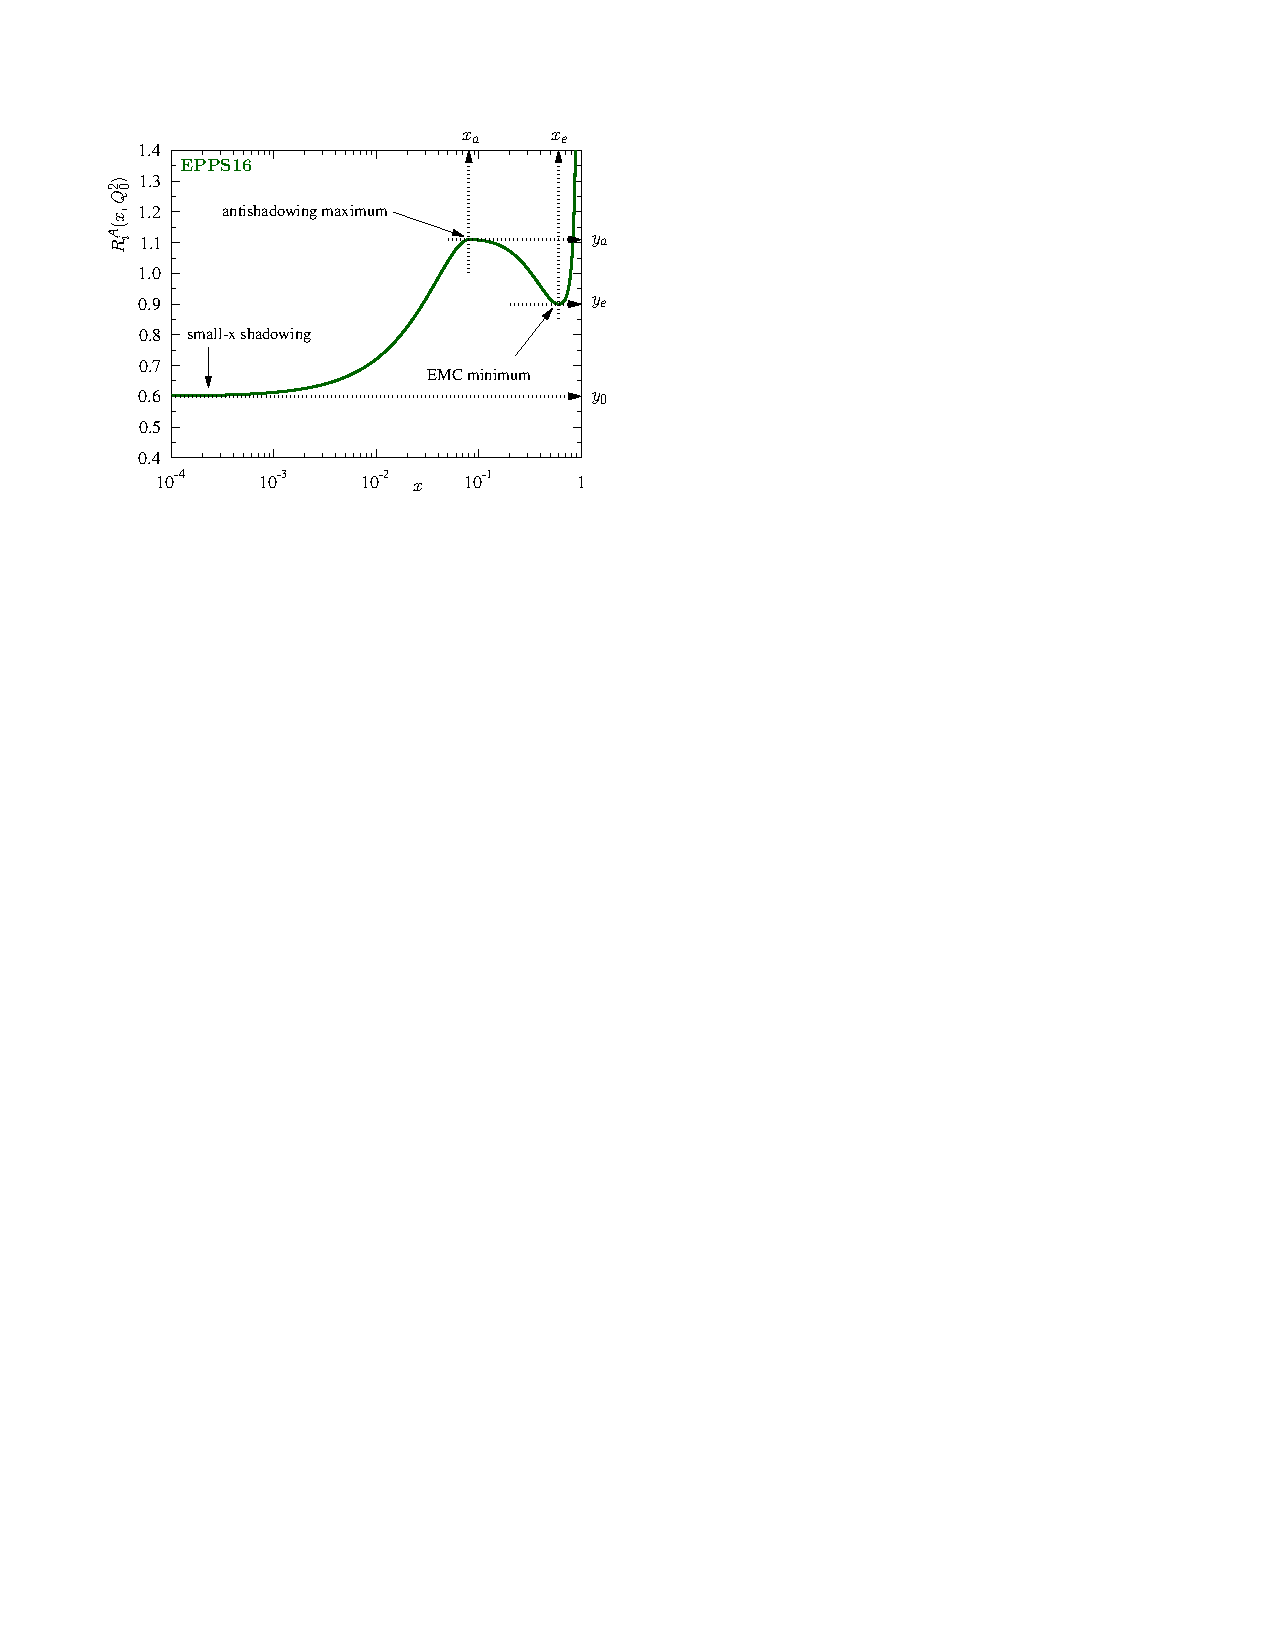
\includegraphics[width=0.8\textwidth]{Introduction/cnm_cartoon}
  \caption{Typical form of PDF modifications in a nucleus\cite{Pumplin2001}.}
  \label{fig:cnm_cartoon}
\end{figure}

The modification in the region where the ratio is less than 1.0 is called ''shadowing'' at very low $x$, and the ''EMC'' effect at  $0.3 < x < 0.7$. The region where the modification is larger than 1.0 is called ''anti-shadowing'' \cite{Pumplin2001}. The exact magnitude of these effects on various measurements, as well as an improved understanding of the nPDF's is a currently under investigation in the field. Recently, a major step forward toward this goal has been the inclusion of LHC pPb data, particularly for extracting the gluon-PDF.
\subsection{Nuclei and Fragmentation}

Aside from differences between the PDFs in free and bound nucleons, there are potential observable effects of the nucleus as a medium itself. Measurements in p+A collisions showed that particle production at moderate transverse momentum increases faster than the number of binary nucleon-nucleon collisions. This was attributed to the Cronin effect where the scattered parton undergoes multiple scatterings in the nucleus, resulting in a transverse momentum boost, \textit{before} the interaction that ultimately produces the final state particle \cite{Cronin1975}.

Currently, however, an open question in the field is the exact timescale of fragmentation, as both pQCD and lattice calculations are unable to provide estimates. This leaves open the possibility that the parton begins to fragment while still inside the nucleus, potentially modifying the fragmentation process and the final state hadrons of the resulting jet.


The current state on cold nuclear matter effects modifying the parton fragmentation function is ambiguous: In di-hadron and direct photon-hadron correlations, no significant modification of the jet fragmentation was observed in measurements by the PHENIX collaboration in d--Au collisions at a center-of-mass energy of 200 GeV~\cite{Adler:2005ad} and the ALICE collaboration in \pPb~collisions at 5.02 TeV~\cite{Acharya:2018edi,Adam:2015xea} at mid rapidity. At forward rapidity, probing a lower-x regime, a strong-modification was observed by the PHENIX collaboration in d-Au collisions~\cite{Adare:2011sc}. A more recent measurement by the PHENIX collaboration with pp, p--Al, and p--Au data revealed a transverse momentum broadening consistent with a path-length dependent effect~\cite{Aidala:2018eqn}. However, a recent ATLAS measurement of the jet fragmentation function in \pPb~collisions showed no evidence for modification of jet fragmentation for jets with $45<\pt<206$ \GeVc~\cite{Aaboud:2017tke}. Measurements of the fragmentation of jets with much lower momentum are necessary to limit the Lorentz boost to the timescales of fragmentation, as such a boost may result in fragmentation outside the nucleus. These measurements would test the $Q^{2}$ evolution of fragmentation functions in cold nuclear matter, testing factorization theorems that are neither proven nor expected to hold in general for collisions involving nuclei~\cite{deFlorian:2011fp}. 

\section{Statement of Purpose}

Parton fragmentation may be modified in the nucleus, offering a way to explore the dynamics of QCD in nuclei including elastic, inelastic, and coherent multiple scattering of partons. Moreover, the known spatial dimensions of nuclei provide a filter possibly shedding light on the timescale of the fragmentation process, which remains unknown~\cite{Accardi:2009qv,Accardi:2012qut}. Additionally, because photons produced in hard scatterings do not strongly interact, they constrain the parton kinematics from the same scattering before any modification. Thus, measurements of photon-tagged jet fragmentation in pA collisions serve as a powerful tool to study multiple-scattering effects in cold nuclear matter~\cite{Xing:2012ii}, which serve as a control for effects of the quark$-$gluon plasma (QGP) in nucleus$-$nucleus collisions, where modifications of the jet spectrum, fragmentation, and substructure have been observed~\cite{Connors:2017ptx}.

In this work, azimuthal correlations of charged hadrons with isolated photons, $\gammaiso$, are analyzed in \pPb~and pp collisions with a center-of-mass energy of \sqrtsNN~ = 5.02 TeV. Isolated photons are measured at midrapidity, {$|\eta|<0.67$}, and with transverse momenta in the range $12 <\pt<40$ \GeVc, which yields the scaling variable {$x_{\mathrm{T}} = 2\pt/\sqrt{s_{\mathrm{NN}}}\ = $ 0.005--0.016}. The kinematic range probed in this analysis offers access to a lower $Q^{2}$ than other LHC experiments, which is where the largest nuclear effects can be expected,  and to a similar $x_{\mathrm{T}}$ range as RHIC measurements at forward rapidity~\cite{Adare:2011sc}. 

Understanding the dynamics of quarks and gluons in nucleons and nuclei is a key goal of modern nuclear physics. Proton$-$nucleus (pA) collisions at high energies provide information about the parton structure of nuclei, parton$-$nucleus interactions, and parton fragmentation in a nuclear medium~\cite{Accardi:2009qv}. The energy of the Large Hadron Collider (LHC) available for pA collisions is a factor of 25 larger than at the Relativistic Heavy Ion Collider (RHIC), and thus it provides unprecedented reach in longitudinal momentum fraction Bjorken-$x$ and $Q^{2}$~\cite{Salgado:2011wc}. 

% The measurement of the transverse momentum of $\gammaiso$ constrains the recoiling parton kinematics in a way that is not possible with inclusive jet production and provides an effective way to probe the nuclear modification of the fragmentation function. Moreover, the per-trigger yield is the ratio of a semi-inclusive cross-section (photon + jet) and inclusive cross-section (photon). Both quantities are sensitive to the nuclear parton distribution functions (PDF) in the same way \cite{kang2016semiinclusive,gamma_cross_section}. Thus, by measuring per-photon quantities, sensitivity to the nuclear PDF is eliminated.
%end
